% =====================================================================
%  Sharpness-Aware Minimization and Its Variants
%  SAM · GSAM · WSAM · Eigen-SAM · X-SAM   (≈ 60 minutes)
%
%  Build:   latexmk -pdf sam-lecture.tex
%  Notes:   pdflatex -jobname=sam-lecture-notes "\def\withnotes{1}\input{sam-lecture.tex}"
% =====================================================================
\documentclass[aspectratio=169,10pt]{beamer}

\usetheme[progressbar=frametitle,numbering=fraction,sectionpage=progressbar,block=fill]{metropolis}
\ifdefined\withnotes
  \setbeameroption{show notes on second screen=right}
\fi

\usepackage[T1]{fontenc}
\usepackage{amsmath,amssymb,bm}
\usepackage{booktabs,array}
\usepackage{tikz}
\usetikzlibrary{arrows.meta,calc,positioning,decorations.pathreplacing}
\usepackage{pgfplots}
\pgfplotsset{compat=1.18}
\usepackage{appendixnumberbeamer}
\usepackage[ruled,vlined,linesnumbered]{algorithm2e}
\SetAlFnt{\small}
\SetAlCapFnt{\small}
\SetKwComment{Comment}{\color{muted}$\triangleright$\ }{}

% ---------------------------------------------------------------- colours
\definecolor{navy}{HTML}{15213B}
\definecolor{sharp}{HTML}{C4651F}
\definecolor{flat}{HTML}{2B62A8}
\definecolor{paper}{HTML}{FAFAF7}
\definecolor{muted}{HTML}{5F6878}
\definecolor{good}{HTML}{2B62A8}

\setbeamercolor{normal text}{fg=navy,bg=paper}
\setbeamercolor{background canvas}{bg=paper}
\setbeamercolor{alerted text}{fg=sharp}
\setbeamercolor{example text}{fg=flat}
\setbeamercolor{frametitle}{bg=navy,fg=paper}
\setbeamercolor{progress bar}{fg=sharp,bg=navy!15}
\setbeamercolor{title separator}{fg=sharp}
\setbeamercolor{block title}{bg=navy!10,fg=navy}
\setbeamercolor{block body}{bg=navy!4,fg=navy}
\setbeamercolor{block title alerted}{bg=sharp!18,fg=navy}
\setbeamercolor{block body alerted}{bg=sharp!6,fg=navy}
\setbeamercolor{block title example}{bg=flat!15,fg=navy}
\setbeamercolor{block body example}{bg=flat!5,fg=navy}
\setbeamercolor{footnote}{fg=muted}
\setbeamercolor{palette primary}{bg=navy,fg=paper}
\setbeamercolor{section title}{fg=navy}
\setbeamertemplate{itemize item}{\color{sharp}\small$\blacktriangleright$}

% section pages: title, progress bar, then one line of paper info
\newcommand{\sectioninfo}{}
\newcommand{\sectionidea}{}
\setbeamertemplate{section page}{%
  \centering
  \begin{minipage}{30em}
    \raggedright
    {\usebeamercolor[fg]{section title}\usebeamerfont{section title}\insertsectionhead}\\[-1ex]
    \usebeamertemplate*{progress bar in section page}
    \par\vspace{0.9em}
    {\small\color{muted}\sectioninfo}\par\vspace{0.6em}
    {\large\itshape\color{navy}\sectionidea}
  \end{minipage}
  \par
}
\newcommand{\partsection}[3]{%
  \renewcommand{\sectioninfo}{#2}%
  \renewcommand{\sectionidea}{#3}%
  \section{#1}}
\setbeamertemplate{itemize subitem}{\color{muted}\scriptsize$\bullet$}

% ---------------------------------------------------------------- macros
\newcommand{\norm}[1]{\lVert #1\rVert}
\newcommand{\fp}{f_{\mathrm{p}}}
\newcommand{\Lsam}{L^{\mathrm{SAM}}}
\newcommand{\sh}[1]{\textcolor{sharp}{#1}}
\newcommand{\fl}[1]{\textcolor{flat}{#1}}
\newcommand{\mt}[1]{\textcolor{muted}{#1}}
\newcommand{\source}[1]{\par\vfill{\scriptsize\mt{#1}}}
\newcommand{\best}[1]{\textbf{#1}}
\newcommand{\paperref}[1]{{\footnotesize\mt{#1}}}
\newcommand{\takeaway}[1]{\begin{beamercolorbox}[sep=7pt,wd=\linewidth]{block body example}#1\end{beamercolorbox}}

% ---------------------------------------------------------------- title
\title{Sharpness-Aware Minimization and Its Variants}
\subtitle{SAM $\cdot$ GSAM $\cdot$ WSAM $\cdot$ Eigen-SAM $\cdot$ X-SAM}
\author{P Sai Aditya}
\date{Flat vs Sharp Minima \quad$|$\quad October 27 \& 29, 2026}

\begin{document}

% =====================================================================
\maketitle
\note{Welcome. One idea today: flat minima generalize better than sharp ones. Five papers, each refining how to find them.
Timing (about 60 min): intro 3, background 6, SAM 13, GSAM 10, WSAM 7, Eigen-SAM 10, X-SAM 8, wrap-up 4.
Colour code used throughout: orange = sharp, blue = flat.}

% =====================================================================
\begin{frame}{Roadmap: five papers, one story}
\centering
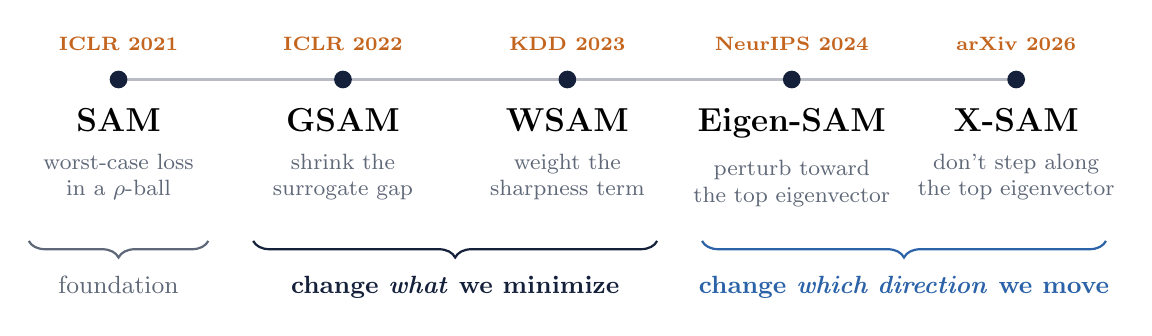
\begin{tikzpicture}[x=2.85cm]
  \draw[navy!30, line width=1.2pt] (0,0) -- (4,0);
  \foreach \i/\yr/\nm/\desc in {
      0/ICLR 2021/SAM/{worst-case loss\\in a $\rho$-ball},
      1/ICLR 2022/GSAM/{shrink the\\surrogate gap},
      2/KDD 2023/WSAM/{weight the\\sharpness term},
      3/NeurIPS 2024/Eigen-SAM/{perturb toward\\the top eigenvector},
      4/arXiv 2026/X-SAM/{don't step along\\the top eigenvector}} {
    \fill[navy] (\i,0) circle (3.2pt);
    \node[above=7pt, font=\scriptsize\bfseries, text=sharp] at (\i,0) {\yr};
    \node[below=7pt, font=\large\bfseries] (n\i) at (\i,0) {\nm};
    \node[below=1pt of n\i, font=\footnotesize, align=center, text=muted] {\desc};
  }
  \draw[decorate, decoration={brace, mirror, amplitude=6pt}, muted, thick]
    (-0.4,-2.05) -- (0.4,-2.05) node[midway, below=9pt, font=\small, text=muted] {foundation};
  \draw[decorate, decoration={brace, mirror, amplitude=6pt}, navy, thick]
    (0.6,-2.05) -- (2.4,-2.05) node[midway, below=9pt, font=\small\bfseries, text=navy] {change \emph{what} we minimize};
  \draw[decorate, decoration={brace, mirror, amplitude=6pt}, flat, thick]
    (2.6,-2.05) -- (4.4,-2.05) node[midway, below=9pt, font=\small\bfseries, text=flat] {change \emph{which direction} we move};
\end{tikzpicture}

\vspace{1.2em}
{\large Same recipe every time: \textbf{perturb} $\to$ \textbf{gradient} $\to$ \textbf{update}.\\[2pt]
\mt{Each paper changes one piece.}}
\end{frame}
\note{Chronological order, and also a story. SAM sets up the recipe. GSAM and WSAM change WHAT is minimized: they pull the sharpness term out and control it. Eigen-SAM and X-SAM change the DIRECTION: Eigen-SAM changes where we perturb, X-SAM how we step; both target the top Hessian eigenvalue. Ask the class: by the end, for any variant, which piece of the recipe did it change?}

% =====================================================================
\partsection{Background}{Flat vs sharp minima, and how we measure sharpness}{Why should flatness help at all?}
% =====================================================================

\begin{frame}{Many minima fit the data. Not all generalize.}
\begin{columns}[T]
\begin{column}{0.56\textwidth}
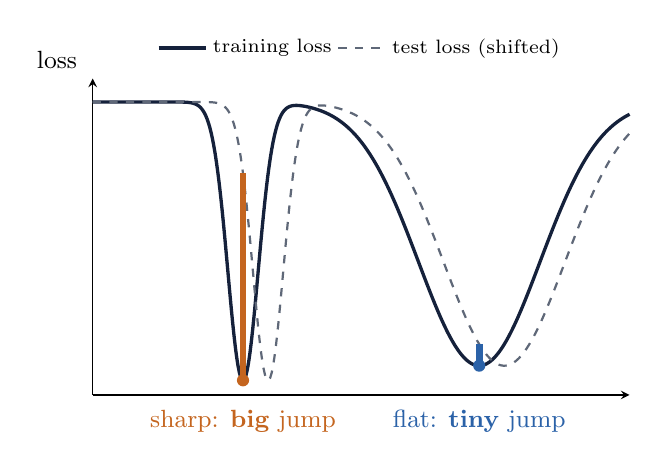
\begin{tikzpicture}
\begin{axis}[width=8.4cm, height=5.6cm, axis lines=left, xtick=\empty, ytick=\empty,
  ylabel={loss},
  ylabel style={font=\small, rotate=-90, at={(ticklabel cs:1)}, anchor=south east},
  xmin=0, xmax=7.5, ymin=0, ymax=1.08, samples=400, domain=0:7.5, clip=false,
  legend style={at={(0.5,1.03)}, anchor=south, legend columns=2, draw=none, fill=none, font=\scriptsize}]
  \addplot[navy, very thick] {1-0.95*exp(-((x-2.1)/0.3)^2)-0.9*exp(-((x-5.4)/1.2)^2)};
  \addplot[muted, thick, dashed] {1-0.95*exp(-((x-2.45)/0.3)^2)-0.9*exp(-((x-5.75)/1.2)^2)};
  \legend{training loss, test loss (shifted)}
  \draw[sharp, line width=2.4pt] (axis cs:2.1,0.05) -- (axis cs:2.1,0.756);
  \draw[flat, line width=2.4pt] (axis cs:5.4,0.10) -- (axis cs:5.4,0.173);
  \fill[sharp] (axis cs:2.1,0.05) circle (2.2pt);
  \fill[flat] (axis cs:5.4,0.10) circle (2.2pt);
  \node[sharp, font=\small, below] at (axis cs:2.1,-0.02) {sharp: \textbf{big} jump};
  \node[flat, font=\small, below] at (axis cs:5.4,-0.02) {flat: \textbf{tiny} jump};
\end{axis}
\end{tikzpicture}
\end{column}
\begin{column}{0.42\textwidth}
\begin{itemize}\setlength{\itemsep}{0.7em}
  \item \textbf{Overparameterized} nets reach $\approx 0$ training loss at many weight settings.
  \item \textbf{Intuition:} the test landscape is the training landscape, slightly shifted.
  \item At a \fl{\textbf{flat}} minimum the shift barely matters; at a \sh{\textbf{sharp}} one the loss shoots up.
\end{itemize}
\end{column}
\end{columns}
\source{Hochreiter \& Schmidhuber (1995, 1997); Keskar et al.\ (2017); Jiang et al.\ (2020): a sharpness measure correlated best with generalization among 40 measures.}
\end{frame}
\note{Picture the loss as a surface over the weights; training walks downhill. Overparameterized nets: many weight settings reach roughly zero training loss, but they behave differently on test data. The dashed curve is the test loss drawn as the training loss nudged sideways. At the sharp minimum the nudge sends the loss way up (orange bar); at the flat minimum it barely moves (blue bar). Notice: the sharp minimum here has slightly LOWER training loss. Keep that in mind for GSAM. Caveat for later: Dinh et al. (2017) showed sharpness can be changed by reparameterization.}

\begin{frame}{Sharpness is curvature: the Hessian}
\begin{columns}[T]
\begin{column}{0.52\textwidth}
\begin{itemize}\setlength{\itemsep}{0.6em}
  \item Hessian $H=\nabla^2 L(w)$: matrix of second derivatives.
  \item Eigenvector $v_i$ = a direction; eigenvalue $\lambda_i$ = how steeply the loss curves along it.
  \item Curvature along any direction $u$:
  \[ \frac{u^\top H u}{\norm{u}^2} \;=\; \sum_i \lambda_i \cos^2\theta_i \]
  \item $\sh{\lambda_1=\lambda_{\max}}$ along $\sh{v_1}$: the sharpest direction, and the standard one-number sharpness measure.
\end{itemize}
\end{column}
\begin{column}{0.46\textwidth}
\begin{exampleblock}{Running example (used in every part)}
\centering
$L(w)=5w_1^2+0.5w_2^2 \;\Rightarrow\; H=\operatorname{diag}(10,\,1)$\\[4pt]
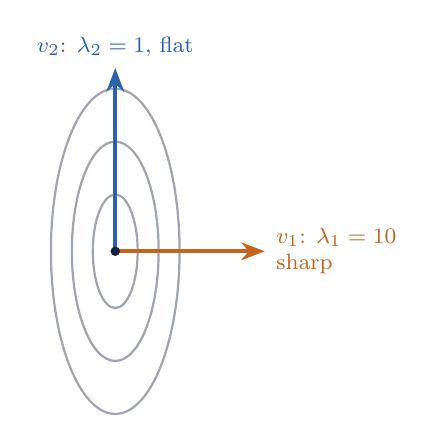
\begin{tikzpicture}[scale=0.95]
  \foreach \k in {0.3,0.58,0.86} \draw[muted!60, thick] (0,0) ellipse ({\k} and {3.16*\k*0.8});
  \draw[-{Stealth[length=3mm]}, sharp, line width=1.6pt] (0,0) -- (2.0,0) node[right, font=\footnotesize, align=left] {$v_1$: $\lambda_1=10$\\sharp};
  \draw[-{Stealth[length=3mm]}, flat, line width=1.6pt] (0,0) -- (0,2.45) node[above, font=\footnotesize] {$v_2$: $\lambda_2=1$, flat};
  \fill[navy] (0,0) circle (1.8pt);
\end{tikzpicture}
\end{exampleblock}
\end{column}
\end{columns}
\end{frame}
\note{Each eigenvector is a direction in weight space; its eigenvalue says how fast the loss curves along it. The boxed formula, u-transpose H u over the squared norm, is the curvature along any direction u, and it equals a weighted sum of eigenvalues by cos-squared of the angles. We will use exactly this to measure "how much sharpness a method sees". Lambda-one is the sharpest direction. Running example: L = 5 w1\textasciicircum{}2 + 0.5 w2\textasciicircum{}2. w1 is the sharp direction (eigenvalue 10), w2 the flat one (eigenvalue 1). Contours are narrow left-right because the loss rises fast that way.}

% =====================================================================
\partsection{Part 1 $\cdot$ SAM}{Foret, Kleiner, Mobahi, Neyshabur $\cdot$ Google Research $\cdot$ ICLR 2021}{Don't just find a low point. Find a low neighbourhood.}
% =====================================================================

\begin{frame}{From a generalization bound to an objective}
\begin{block}{Theorem 1 (informal). With high probability over the training set $S$:}
\[
L_{\mathcal D}(w) \;\le\; \max_{\norm{\epsilon}_2\le\rho} L_S(w+\epsilon) \;+\; h\!\left(\norm{w}_2^2/\rho^2\right),
\qquad h \text{ strictly increasing}
\]
\end{block}
Rewrite the right-hand side to expose sharpness:
\[
\underbrace{\Big[\max_{\norm{\epsilon}_2\le\rho} L_S(w+\epsilon) - L_S(w)\Big]}_{\textstyle\sh{\text{sharpness}}}
\;+\; \underbrace{L_S(w)}_{\text{training loss}}
\;+\; \underbrace{h(\norm{w}_2^2/\rho^2)}_{\to\ \lambda\norm{w}_2^2\ \text{(weight decay)}}
\]
\begin{alertblock}{The SAM objective (Eq.\ 1)}
\[
\min_w \; L_S^{\mathrm{SAM}}(w) + \lambda\norm{w}_2^2,
\qquad
L_S^{\mathrm{SAM}}(w) \triangleq \max_{\norm{\epsilon}_p\le\rho} L_S(w+\epsilon)
\]
\end{alertblock}
\source{PAC-Bayes proof in App.\ A; assumes Gaussian weight noise does not lower test loss. $p=2$ works best (App.\ C.5).}
\end{frame}
\note{L\_S = training loss, L\_D = true population loss. The bound: true loss is at most the WORST training loss in a radius-rho ball, plus a weight-norm term. Rewrite: [max nearby minus loss here] is the sharpness. So: keep loss low, sharpness low, weights small. h is an artefact of the proof, so it becomes ordinary L2 regularization. Result: a min-max problem. The inner max finds the worst neighbour; the outer min pushes it down. Proof idea if asked: PAC-Bayes with Gaussian posterior N(w, sigma\textasciicircum{}2 I), Gaussian prior at zero, prior variance from a fixed grid plus union bound; chi-square concentration puts the Gaussian perturbation inside the rho-ball w.h.p. Full statement in the backup slides.}

\begin{frame}{Making the min-max cheap: three approximations}
\begin{enumerate}\setlength{\itemsep}{0.9em}
  \item \textbf{Linearize the inner max} (first-order Taylor around $\epsilon=0$):
  \[ \epsilon^*(w) \approx \arg\max_{\norm{\epsilon}_p\le\rho}\; \epsilon^\top \nabla L_S(w) \]
  \item \textbf{Solve it exactly} (dual norm, $\tfrac1p+\tfrac1q=1$). For $p=2$:
  \[ \hat\epsilon(w)=\rho\,\frac{\nabla L_S(w)}{\norm{\nabla L_S(w)}_2}
     \qquad\mt{\text{climb distance $\rho$ straight up the gradient}} \]
  \item \textbf{Drop the Hessian term} from the chain rule:
  \[ \nabla \Lsam_S(w) \approx \nabla L_S(w)\big|_{w+\hat\epsilon}
     + \underbrace{\tfrac{d\hat\epsilon}{dw}\nabla L_S(w)\big|_{w+\hat\epsilon}}_{\text{dropped}}
     \;\;\Rightarrow\;\; \boxed{\nabla \Lsam_S(w)\approx \nabla L_S(w+\hat\epsilon)} \]
\end{enumerate}
\begin{alertblock}{Surprise (App.\ C.4)}
Keeping the second-order term made test error \emph{worse}. The authors call the cause unclear.
\end{alertblock}
\end{frame}
\note{The exact max over a ball is intractable for a deep net. (1) Taylor-expand; the constant drops out, leaving a dot product under a norm constraint. (2) Dual-norm solution; for p = 2, just rescale the gradient to length rho. That is the approximate worst neighbour. p = infinity gives rho*sign(grad), the FGSM form; p = 1 would perturb a single weight. (3) epsilon-hat depends on w, so the chain rule gives a Hessian term. Computable with Hessian-vector products, but dropped for speed. Final rule: gradient AT the perturbed point, applied AT the original point. App. C.4: WRN-40x2 on CIFAR-10: early in training the two update directions have cosine near 1; near convergence they diverge; the first-order version reaches lower test error. Unexplained, good discussion point.}

\begin{frame}{One SAM step = two gradient computations}
\begin{columns}[c]
\begin{column}{0.54\textwidth}
\begin{algorithm}[H]
\caption{SAM (base optimizer: SGD)}
\KwIn{data $S$, step size $\eta$, radius $\rho$}
\For{$t=0,1,2,\dots$}{
  sample mini-batch $\mathcal B$\;
  $g \leftarrow \nabla L_{\mathcal B}(w_t)$ \Comment*[r]{pass 1}
  $\hat\epsilon \leftarrow \rho\, g/\norm{g}$ \Comment*[r]{climb}
  $g_{\mathrm{SAM}} \leftarrow \nabla L_{\mathcal B}(w_t+\hat\epsilon)$ \Comment*[r]{pass 2}
  $w_{t+1} \leftarrow w_t - \eta\, g_{\mathrm{SAM}}$ \Comment*[r]{from $w_t$}
}
\end{algorithm}
\end{column}
\begin{column}{0.44\textwidth}
\centering
\begin{tikzpicture}[scale=0.95, >={Stealth[length=2.6mm]}]
  \coordinate (w) at (0,0);
  \coordinate (wa) at (1.7,1.25);
  \draw[->, sharp, very thick, dashed] (w) -- (wa) node[midway, above left, font=\scriptsize] {$\hat\epsilon$};
  \draw[->, navy, very thick] (wa) -- ++(0.55,1.35) node[right, font=\scriptsize] {$\nabla L(w_t+\hat\epsilon)$};
  \draw[->, muted, very thick] (w) -- (-1.75,-1.3) node[left, font=\scriptsize] {SGD step};
  \draw[->, flat, very thick] (w) -- (-0.62,-1.55) node[below, font=\scriptsize] {SAM step};
  \fill[navy] (w) circle (2.2pt) node[right=3pt, font=\scriptsize] {$w_t$};
  \fill[sharp] (wa) circle (2.2pt) node[right=3pt, font=\scriptsize] {$w_t+\hat\epsilon$};
\end{tikzpicture}
\end{column}
\end{columns}
\vspace{0.4em}
\begin{itemize}
  \item Cost: \textbf{$2\times$ SGD} per step. Wraps any base optimizer (SGD, Adam, \dots).
  \item Multi-GPU: each device computes its own $\hat\epsilon$ on its slice; the SAM gradients are averaged.
\end{itemize}
\end{frame}
\note{Walk through the five lines. Stress: the gradient is computed at the perturbed point (orange) but the step is taken from the original point w\_t. The figure (Fig. 2 of the paper, redrawn): the SGD step goes along minus the local gradient; the SAM step uses the gradient from the worst neighbour, which bends it away from sharp regions. Two backprops per step means 2x cost. Multi-GPU detail matters later: m-sharpness.}

\begin{frame}{Running example: SAM pushes harder on the sharp direction}
\begin{columns}[T]
\begin{column}{0.5\textwidth}
$L=5w_1^2+0.5w_2^2$, \; $w=(1,1)$, \; $\rho=0.1$\\[6pt]
\renewcommand{\arraystretch}{1.25}
\begin{tabular}{@{}ll@{}}
\toprule
Gradient at $w$ & $(10,\;1)$ \\
$\hat\epsilon=\rho g/\norm{g}$ & $(0.0995,\;0.00995)$ \\
Perturbed point $w+\hat\epsilon$ & $(1.0995,\;1.00995)$ \\
SAM gradient & $(10.995,\;1.010)$ \\
\bottomrule
\end{tabular}
\end{column}
\begin{column}{0.48\textwidth}
\begin{block}{Compared with plain SGD}
\sh{\textbf{Sharp} direction $w_1$}: $10 \to 10.995$ \quad \sh{\textbf{+10\%}}\\[3pt]
\fl{\textbf{Flat} direction $w_2$}: \;$1 \to 1.010$ \quad\;\, \fl{\textbf{+1\%}}
\end{block}
\vspace{0.3em}
Why, to first order:
\[ \nabla L(w+\hat\epsilon) \approx \nabla L(w) + \rho\,\frac{H\,\nabla L(w)}{\norm{\nabla L(w)}} \]
\mt{\small The Hessian amplifies the sharp directions.}
\end{column}
\end{columns}
\vspace{0.6em}
\begin{alertblock}{Keep this in mind}
SAM only ``sees'' curvature \emph{along the gradient direction}. If $\nabla L$ is not aligned with $v_1$, the effect is weak. \mt{(Parts 4--5.)}
\end{alertblock}
\end{frame}
\note{This is my own worked example, not from the paper. At (1,1) the gradient is (10,1). The perturbation is a step of 0.1 along it. The gradient at the perturbed point grows by 10\% in the sharp direction but only 1\% in the flat one. The first-order expansion shows why: the extra term is the Hessian times the gradient direction. This is the hook for later: SAM only attacks sharpness in the direction the gradient happens to point.}

\begin{frame}{Experiments: setup}
\begin{itemize}\setlength{\itemsep}{0.55em}
  \item \textbf{Only the optimizer changes}: existing training recipes kept, SGD swapped for SAM.
  \item $\rho$ grid $\{0.01, 0.02, 0.05, 0.1, 0.2, 0.5\}$, tuned on 10\% held-out training data. \;$\rho=0.05$ is a solid default (App.\ C.3).
  \item \textbf{Fair compute}: SGD may run $2\times$ the epochs; its best result is reported.
  \item 5 runs per setting; mean $\pm$ 95\% CI. \;JAX, $8\times$ V100 (CIFAR); TPUv3 (ImageNet).
  \item Models: WideResNet-28-10, Shake-Shake 26 2$\times$96d, PyramidNet ($+$ShakeDrop); ResNet-50/101/152; EfficientNet-B7/L2; ResNet-32.
  \item Tasks: CIFAR-10/100, SVHN, Fashion-MNIST, ImageNet, 9 fine-tuning datasets, noisy labels.
\end{itemize}
\end{frame}
\note{Emphasise the fairness choices: same recipe, SGD gets twice the epochs, 5 seeds with confidence intervals. rho = 0.05 rerun everywhere without tuning (App. C.3) still keeps most gains, so the method is not fragile. CIFAR batch 256; learning rate and weight decay grid-searched first without SAM.}

\begin{frame}{Results: CIFAR and ImageNet (test error, \%)}
\begin{columns}[T]
\begin{column}{0.55\textwidth}
\centering\footnotesize
\textbf{CIFAR} \mt{(selected rows of Table 1)}\\[3pt]
\begin{tabular}{@{}lcccc@{}}
\toprule
& \multicolumn{2}{c}{CIFAR-10} & \multicolumn{2}{c}{CIFAR-100}\\
\cmidrule(lr){2-3}\cmidrule(lr){4-5}
Model (aug.) & SGD & SAM & SGD & SAM \\
\midrule
WRN-28-10, 1800 ep (AA) & 2.2 & \best{1.6} & 16.1 & \best{12.8}\\
Shake-Shake (AA) & 1.9 & \best{1.6} & 14.1 & \best{12.8}\\
PyramidNet (basic) & 4.0 & \best{2.7} & 19.7 & \best{14.6}\\
PyramidNet+SD (AA) & 1.6 & \best{1.4} & 10.6 & \best{10.3}\\
\bottomrule
\end{tabular}
\end{column}
\begin{column}{0.42\textwidth}
\centering\footnotesize
\textbf{ImageNet, top-1} \mt{(Table 2)}\\[3pt]
\begin{tabular}{@{}lccc@{}}
\toprule
Model & Epochs & SGD & SAM\\
\midrule
ResNet-50 & 400 & 22.3 & \best{20.9}\\
ResNet-101 & 200 & 20.9 & \best{19.4}\\
ResNet-101 & 400 & 22.3 & \best{19.0}\\
ResNet-152 & 400 & 20.9 & \best{18.4}\\
\bottomrule
\end{tabular}
\end{column}
\end{columns}
\vspace{0.8em}
\begin{itemize}
  \item SAM improved \textbf{every} CIFAR setting; 10.3\% on CIFAR-100 was SOTA without extra data.
  \item ImageNet: SGD \sh{overfits} from 200 to 400 epochs; SAM keeps improving.
\end{itemize}
\source{AA = AutoAugment; SD = ShakeDrop. SVHN 0.99\% and Fashion-MNIST 3.59\% error (App.\ B.1).}
\end{frame}
\note{Pick two headline numbers: WRN with AutoAugment on CIFAR-10 goes 2.2 to 1.6; with SAM a simple WRN matches gains that previously needed complex architectures. ImageNet: ResNet-152 20.3 to 18.4 at 200 epochs, 18.4 at 400. The overfitting observation is important: ResNet-101 with SGD gets worse from 20.9 to 22.3 when trained longer, SAM improves from 19.4 to 19.0.}

\begin{frame}{Results: fine-tuning and label noise}
\begin{columns}[T]
\begin{column}{0.42\textwidth}
\centering\small
\textbf{Fine-tuning EfficientNet-L2} \mt{(error, \%)}\\[3pt]
\begin{tabular}{@{}lcc@{}}
\toprule
Dataset & no SAM & SAM\\
\midrule
CIFAR-10 & 0.34 & \best{0.30}\\
CIFAR-100 & 4.07 & \best{3.92}\\
ImageNet & 11.8 & \best{11.39}\\
\bottomrule
\end{tabular}\\[4pt]
\mt{\scriptsize SAM improved all 9 datasets; ImageNet beat ViT's 11.45.}
\end{column}
\begin{column}{0.56\textwidth}
\centering\small
\textbf{CIFAR-10 with noisy labels} \mt{(clean test acc., \%)}\\[3pt]
\begin{tabular}{@{}lcccc@{}}
\toprule
Noise rate & 20 & 40 & 60 & 80\\
\midrule
SGD & 84.8 & 68.8 & 48.2 & 26.2\\
Mixup & 93.0 & 90.0 & 83.8 & 70.2\\
\textbf{SAM} & \best{95.1} & \best{93.4} & \best{90.5} & \best{77.9}\\
Bootstrap + SAM & 95.4 & 94.2 & 91.8 & 79.9\\
\mt{MentorMix (lit.)} & \mt{95.6} & \mt{94.2} & \mt{91.3} & \mt{81.0}\\
\bottomrule
\end{tabular}
\end{column}
\end{columns}
\vspace{0.8em}
\begin{exampleblock}{Robustness for free}
Plain SAM, with no noise-specific tricks, beats every dedicated noisy-label method except MentorMix.
\end{exampleblock}
\source{ResNet-32, 200 epochs; $\rho=0.1$ ($0.05$ at 80\% noise). Bootstrap: retrain on the first model's predicted labels.}
\end{frame}
\note{Fine-tuning: EfficientNet-B7 (ImageNet only) and L2 (ImageNet + JFT, NoisyStudent, 475 px). SAM improves all nine datasets, new SOTA on several. Label noise: a fraction of training labels randomly flipped, test set clean. Intuition: noisy labels perturb the loss landscape, and SAM seeks solutions robust to perturbation. Bootstrapped SAM comes close to MentorMix, which is far more complex.}

\begin{frame}{What SAM actually finds}
\begin{columns}[T]
\begin{column}{0.48\textwidth}
\begin{block}{Hessian spectrum at convergence}
\centering
\renewcommand{\arraystretch}{1.3}
\begin{tabular}{@{}lcc@{}}
& SGD & SAM\\
\midrule
$\lambda_{\max}$ & $\approx 24$ & \fl{\textbf{$\approx 1.0$}}\\
$\lambda_{\max}/\lambda_5$ & up to 11.4 & \fl{\textbf{2.6}}\\
\end{tabular}\\[4pt]
\mt{\scriptsize WRN-40-10, CIFAR-10, no batch norm; Lanczos estimate.}
\end{block}
\mt{\small Remember $\lambda_{\max}$: GSAM, Eigen-SAM and X-SAM all target it.}
\end{column}
\begin{column}{0.5\textwidth}
\begin{block}{$m$-sharpness}
In practice $\hat\epsilon$ is computed per device on $m$ examples, not on the whole training set.
\begin{itemize}
  \item Smaller $m$ $\Rightarrow$ \textbf{better test error}.
  \item Smaller $m$ $\Rightarrow$ $m$-sharpness \textbf{predicts the generalization gap better}.
\end{itemize}
\end{block}
\mt{\small So the full-dataset sharpness in Theorem 1 is not the most predictive quantity.}
\end{column}
\end{columns}
\end{frame}
\note{Hessian spectra (Fig. 3 left): SAM really lands in lower-curvature minima; lambda-max drops from about 24 to about 1. Batch norm removed because it obscures Hessian interpretation. m-sharpness: computing the perturbation per accelerator is equivalent to a sum of independent worst-case perturbations on groups of m points. Smaller m generalizes better, which conveniently fits data parallelism; that is why the authors recommend NOT syncing perturbations. Measured with the Jiang et al. framework on the NeurIPS 2020 Predicting Generalization tasks.}

\begin{frame}{Ablations, and what SAM left open}
\begin{columns}[T]
\begin{column}{0.56\textwidth}
\small
\renewcommand{\arraystretch}{1.2}
\begin{tabular}{@{}>{\raggedright}p{2.4cm}>{\raggedright\arraybackslash}p{4.9cm}@{}}
\toprule
Ablation & Finding\\
\midrule
2nd-order term (C.4) & Worse test error; cause unexplained\\
Choice of $p$ (C.5) & Adversarial $\epsilon$ beats random noise; $p=2$ beats $p=\infty$\\
Inner steps (C.6) & 1 step is accurate most of training; 5 steps find $\sim$3\% higher loss near the end; test error barely changes\\
Fixed $\rho=0.05$ (C.3) & Gains largely preserved\\
\bottomrule
\end{tabular}
\end{column}
\begin{column}{0.42\textwidth}
\begin{alertblock}{Open problems}
\begin{itemize}
  \item $2\times$ compute per step
  \item Low worst-case loss $\neq$ flat minimum\\ \mt{$\to$ GSAM}
  \item Fixed 1:1 loss/sharpness balance\\ \mt{$\to$ WSAM}
  \item Only sees curvature along $\nabla L$\\ \mt{$\to$ Eigen-SAM, X-SAM}
\end{itemize}
\end{alertblock}
\end{column}
\end{columns}
\end{frame}
\note{Ablations are often skipped, so they make you stand out. Random perturbations of the same norm work worse than adversarial ones, so the worst case matters. Multiple inner ascent steps: on CIFAR-100, several steps are slightly but significantly better. Open problems on the right: the first is stated in the paper; the others were identified by the later papers, and each points to the next part. Small catch in App. C.5: the p = 2 formula there has the norm squared in the denominator; it should be the plain norm, as in the main text.}

% =====================================================================
\partsection{Part 2 $\cdot$ GSAM}{Zhuang, Gong, Yuan, Cui, Adam, Dvornek, Tatikonda, Duncan, Liu $\cdot$ Yale \& Google $\cdot$ ICLR 2022}{A low worst-case loss can still be sharp.}
% =====================================================================

\begin{frame}{A low perturbed loss does not mean a flat minimum}
\begin{columns}[c]
\begin{column}{0.57\textwidth}
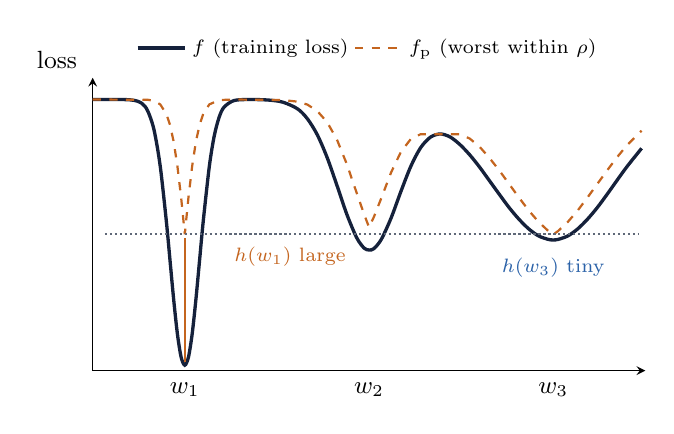
\begin{tikzpicture}
\begin{axis}[width=8.6cm, height=5.3cm, axis lines=left, xtick=\empty, ytick=\empty,
  ylabel={loss}, ylabel style={font=\small, rotate=-90, at={(ticklabel cs:1)}, anchor=south east},
  xmin=0.2, xmax=9.2, ymin=0, ymax=1.08, clip=false,
  legend style={at={(0.5,1.03)}, anchor=south, legend columns=2, draw=none, fill=none, font=\scriptsize}]
\addplot[navy, very thick, smooth] coordinates {(0.20,1.000) (0.80,0.999) (1.00,0.986) (1.10,0.956) (1.20,0.887) (1.30,0.754) (1.40,0.550) (1.46,0.405) (1.52,0.260) (1.58,0.135) (1.64,0.050) (1.70,0.020) (1.76,0.050) (1.82,0.135) (1.88,0.260) (1.94,0.405) (2.00,0.550) (2.10,0.754) (2.18,0.866) (2.26,0.935) (2.34,0.972) (2.50,0.996) (2.74,1.000) (3.06,0.998) (3.30,0.990) (3.54,0.965) (3.70,0.928) (3.86,0.869) (4.02,0.785) (4.18,0.682) (4.34,0.576) (4.50,0.490) (4.62,0.452) (4.70,0.445) (4.78,0.450) (4.90,0.484) (5.06,0.563) (5.22,0.661) (5.38,0.753) (5.54,0.822) (5.70,0.861) (5.86,0.873) (6.02,0.862) (6.18,0.834) (6.34,0.796) (6.50,0.751) (6.66,0.701) (6.82,0.651) (6.98,0.602) (7.14,0.559) (7.30,0.523) (7.46,0.497) (7.62,0.484) (7.70,0.482) (7.78,0.484) (7.94,0.497) (8.10,0.523) (8.26,0.559) (8.42,0.602) (8.58,0.651) (8.74,0.702) (8.90,0.752) (9.14,0.820)};
\addplot[sharp, thick, dashed] coordinates {(0.20,1.000) (1.10,0.999) (1.20,0.995) (1.30,0.982) (1.40,0.947) (1.46,0.906) (1.52,0.843) (1.58,0.754) (1.64,0.639) (1.70,0.503) (1.76,0.639) (1.82,0.754) (1.88,0.843) (1.94,0.906) (2.00,0.947) (2.10,0.982) (2.26,0.998) (2.50,1.000) (3.30,0.998) (3.54,0.992) (3.70,0.981) (3.86,0.957) (4.02,0.916) (4.18,0.851) (4.34,0.761) (4.50,0.655) (4.62,0.577) (4.70,0.529) (4.78,0.567) (4.90,0.636) (5.06,0.731) (5.22,0.807) (5.38,0.854) (5.54,0.872) (6.18,0.872) (6.34,0.856) (6.50,0.826) (6.66,0.785) (6.82,0.739) (6.98,0.689) (7.14,0.639) (7.30,0.591) (7.46,0.549) (7.62,0.515) (7.70,0.502) (7.78,0.515) (7.94,0.549) (8.10,0.591) (8.26,0.639) (8.42,0.689) (8.58,0.739) (8.74,0.787) (8.90,0.831) (9.14,0.885)};
\legend{$f$ (training loss), $f_{\mathrm p}$ (worst within $\rho$)}
\draw[muted, densely dotted, thick] (axis cs:0.4,0.503) -- (axis cs:9.1,0.503);
\node[font=\small, below] at (axis cs:1.70,-0.01) {$w_1$};
\node[font=\small, below] at (axis cs:4.70,-0.01) {$w_2$};
\node[font=\small, below] at (axis cs:7.70,-0.01) {$w_3$};
\node[font=\scriptsize, sharp, anchor=west] at (axis cs:2.35,0.42) {$h(w_1)$ large};
\draw[sharp, thick] (axis cs:1.70,0.03) -- (axis cs:1.70,0.49);
\node[font=\scriptsize, flat, anchor=north] at (axis cs:7.70,0.45) {$h(w_3)$ tiny};
\end{axis}
\end{tikzpicture}
\end{column}
\begin{column}{0.41\textwidth}
At a minimum ($\nabla f=0$), Taylor gives
\[ \fp(w) \approx \underbrace{f(w)}_{\text{depth}} + \underbrace{\tfrac12\rho^2\sigma_{\max}}_{\text{sharpness}} \]
$\fp$ mixes the two.\\[6pt]
In the plot: $\fp(w_1)\approx\fp(w_3)<\fp(w_2)$\\
\mt{$\Rightarrow$ SAM can't tell sharp $w_1$ from flat $w_3$.}\\[6pt]
The \textbf{gap} $h=\fp-f$ ranks them correctly:\\
$h(w_1)>h(w_2)>h(w_3)$.
\end{column}
\end{columns}
\source{Lemma 3.1: for two minima, $\fp(w_1)\le\fp(w_2)$ does \emph{not} imply $\sigma_{\max}(w_1)\le\sigma_{\max}(w_2)$. Figure redrawn after the paper's Fig.\ 1.}
\end{frame}
\note{The opening question: does minimizing the worst-case loss always find a flat minimum? No. Near a minimum f\_p is depth plus half rho-squared sigma-max. A minimum can have low f\_p because it is flat, OR because it is very deep even though sharp. Think of f\_p as a max-pooled version of f with window 2*rho. In this plot (my recreation of their Fig. 1): w1 is a deep narrow valley, w3 a shallow wide one; their f\_p values are equal (dotted line), so SAM is equally happy at both. The gap h orders them correctly. Some PDF extractions drop the negation in Lemma 3.1; the proof makes clear it says "does not imply".}

\begin{frame}{The surrogate gap measures sharpness}
\begin{block}{Definition (Eq.\ 4)}
\[ h(w) \triangleq \fp(w) - f(w) \;\approx\; f(w^{\mathrm{adv}}) - f(w),
\qquad w^{\mathrm{adv}} = w + \rho\,\frac{\nabla f(w)}{\norm{\nabla f(w)}+\epsilon} \]
\end{block}
\begin{columns}[T]
\begin{column}{0.48\textwidth}
\begin{exampleblock}{Lemma 3.2 \;(non-negative)}
For small $\rho$: $h(w)\approx\rho\norm{\nabla f(w)}\ge 0$ for all $w$.
\end{exampleblock}
\end{column}
\begin{column}{0.48\textwidth}
\begin{alertblock}{Lemma 3.3 \;(it \emph{is} the top eigenvalue)}
At a local minimum $w^*$, small $\rho$:
\[ \sigma_{\max} \approx \frac{2\,h(w^*)}{\rho^2} \]
\end{alertblock}
\end{column}
\end{columns}
\vspace{0.4em}
\begin{itemize}
  \item Smaller $h$ $\Rightarrow$ flatter minimum. \;So \textbf{minimize $h$}.
  \item Free to compute: SAM already evaluates $f(w)$ and $f(w^{\mathrm{adv}})$.
  \item \mt{Subtlety: away from a minimum, $h$ mostly tracks $\norm{\nabla f}$, not curvature.}
\end{itemize}
\end{frame}
\note{h is exactly the sharpness bracket from SAM's Theorem 1, promoted to its own objective. Lemma 3.2: to first order h is rho times the gradient norm, non-negative. Lemma 3.3: at a minimum the gradient vanishes, the quadratic term remains, and h is half rho-squared sigma-max. The subtlety (follows from the two proofs, not stressed in the paper): far from a minimum, h mostly measures gradient norm; it is a faithful sharpness measure mainly late in training. epsilon = 1e-12 avoids division by zero.}

\begin{frame}{Lower the gap without touching the worst-case loss}
\begin{columns}[c]
\begin{column}{0.45\textwidth}
\centering
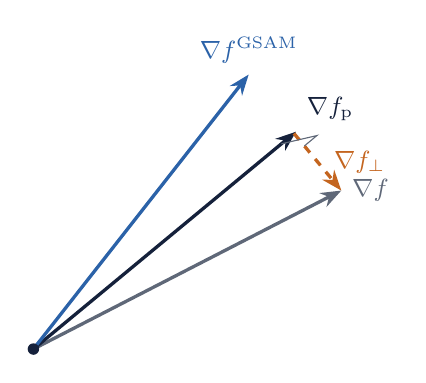
\begin{tikzpicture}[scale=1.15, >={Stealth[length=2.6mm]}]
  \coordinate (O) at (0,0);
  \coordinate (gp) at (2.9,2.4);
  \coordinate (g) at (3.4,1.75);
  \coordinate (par) at (2.877,2.381);
  \coordinate (gs) at (2.377,3.031);
  \draw[->, muted, very thick] (O) -- (g) node[right, font=\small] {$\nabla f$};
  \draw[->, navy, very thick] (O) -- (gp) node[above right, font=\small] {$\nabla \fp$};
  \draw[->, sharp, very thick, dashed] (par) -- (g) node[midway, right=2pt, font=\small] {$\nabla f_\perp$};
  \draw[->, flat, very thick] (O) -- (gs) node[above, font=\small] {$\nabla f^{\mathrm{GSAM}}$};
  \draw[muted] ($(par)!0.18cm!(g)$) -- ($($(par)!0.18cm!(g)$)!0.18cm!90:(g)$) -- ($(par)!0.18cm!(O)$);
  \fill[navy] (O) circle (1.8pt);
\end{tikzpicture}\\[2pt]
{\small $\nabla f^{\mathrm{GSAM}} = \nabla\fp - \alpha\,\nabla f_\perp$}
\end{column}
\begin{column}{0.53\textwidth}
\textbf{Why not $\min \fp + \lambda h$?} \;$\nabla h$ can point \emph{against} $\nabla\fp$, so reducing $h$ would raise $\fp$.\\[2pt]
\mt{\small ViT-B/32 ImageNet: 75.4\% vs GSAM 76.8\% (Table 2).}\\[8pt]
\textbf{Decompose} $\nabla f$ relative to $\nabla\fp$:
\begin{enumerate}
  \item $\nabla h = \nabla\fp - \nabla f$
  \item $\nabla\fp$ has no component $\perp$ to itself
  \item so $\nabla h_\perp = -\nabla f_\perp$
\end{enumerate}
\vspace{4pt}
Step along $+\nabla f_\perp$: \;$f$ \textbf{rises}, $\fp$ \textbf{unchanged} $\Rightarrow$ $h$ \textbf{shrinks}.\\[3pt]
\mt{\small\itshape The ceiling stays put, the floor rises: a shallower valley.}
\end{column}
\end{columns}
\end{frame}
\note{The core trick. First, why not just add lambda*h? Gradient conflict, shown by the paper's Fig. 2 and confirmed in Table 2. Design principle: f\_p is primary ("a flat solution with high loss is meaningless"), and reducing h must never increase f\_p. Derivation in three lines. Moving along the orthogonal direction does not change f\_p to first order. A descent step on h there equals an ascent step on f. f goes up, f\_p stays, so h = f\_p - f shrinks. Note that the GSAM direction and grad f always lie on opposite sides of grad f\_p.}

\begin{frame}{GSAM in practice: three extra lines}
\begin{columns}[T]
\begin{column}{0.52\textwidth}
\begin{algorithm}[H]
\caption{GSAM}
\For{$t=1,\dots,T$}{
  $\rho_t \leftarrow \rho_{\min} + (\rho_{\max}-\rho_{\min})\frac{\mathrm{lr}_t-\mathrm{lr}_{\min}}{\mathrm{lr}_{\max}-\mathrm{lr}_{\min}}$\;
  $g \leftarrow \nabla f(w_t)$;\; $w^{\mathrm{adv}} \leftarrow w_t + \rho_t\, g/(\norm{g}+\epsilon)$\;
  $g_p \leftarrow \nabla f(w^{\mathrm{adv}})$\;
  $g_\parallel \leftarrow \frac{\langle g,g_p\rangle}{\norm{g_p}^2}\,g_p$;\; $g_\perp \leftarrow g - g_\parallel$\;
  $w_{t+1} \leftarrow w_t - \eta_t\,(g_p - \alpha\, g_\perp)$\;
}
\end{algorithm}
\mt{\small Same 2 backprops as SAM; projection is one dot product.}
\end{column}
\begin{column}{0.46\textwidth}
\textbf{Running example} \mt{\small($w=(1,1)$, $\rho=0.1$, $\alpha=1$)}\\[4pt]
\small
\renewcommand{\arraystretch}{1.2}
\begin{tabular}{@{}ll@{}}
\toprule
$g$ & $(10,\;1)$\\
$g_p$ & $(10.995,\;1.010)$\\
$g_\perp$ & $(-0.007,\;0.081)$\\
check $g_\perp\cdot g_p$ & $\approx 0$\\
GSAM step & $(11.002,\;0.929)$\\
\bottomrule
\end{tabular}\\[8pt]
Sharp-to-flat push ratio:\\[2pt]
SGD \textbf{10.0} \;$\to$\; SAM \textbf{10.9} \;$\to$\; GSAM \textbf{11.8}
\end{column}
\end{columns}
\end{frame}
\note{Line 1 is new: rho follows the learning-rate schedule, needed for the convergence proof. The ablation will show the schedule is not where the gain comes from. Cost is essentially SAM's. Toy example (mine): the orthogonal component is tiny in 2-D, but it shifts the step further toward the sharp axis. In high dimensions g\_perp is much richer.}

\begin{frame}{GSAM theory}
\begin{block}{Theorem 5.1 (convergence)}
Non-convex $L$-smooth $f$, bounded noisy gradients $\norm{g^{(t)}}\le G$, $\eta_t=\eta_0/\sqrt t$, $\rho_t\propto\eta_t$:
\[ \tfrac1T\textstyle\sum_t \mathbb E\norm{\nabla\fp(w_t)}^2 \le \frac{C_1+C_2\log T}{\sqrt T},
\qquad \tfrac1T\sum_t \mathbb E\norm{\nabla f(w_t)}^2 \le \frac{C_3+C_4\log T}{\sqrt T} \]
\end{block}
\begin{block}{Corollary 5.2.1 (PAC-Bayes)}
\[ \mathbb E[\text{test loss}] \le \hat h + \underbrace{\hat f(w)}_{\text{train loss}} + 4\sqrt{\big(KL(\mathcal Q\Vert\mathcal P)+\log\tfrac{2m}{a}\big)/m} \]
\end{block}
\begin{alertblock}{Theorem 5.3 (GSAM shrinks $h$ beyond SAM)}
\[ \frac{\alpha c^2\rho_0^2\eta_0|\sigma|_{\min}^2}{G^2} \;\le\; \lim_{T\to\infty}\textstyle\sum_{t}\Delta\hat h_t \;\le\; 2.7\,\alpha L^2\eta_0\rho_0^2 \]
\end{alertblock}
\end{frame}
\note{Convergence: O(log T / sqrt T), like Adam-type optimizers. The ascent term contributes zero in expectation to f\_p's descent, because g\_perp is orthogonal to grad f\_p. Corollary: smaller surrogate gap gives a tighter bound. App. A.7 argument: f\_p = C + h only matches the bound if rho\_train equals the unknown "true" rho; usually rho\_true > rho\_train (test points lie outside the training convex hull; people pick small rho), so a low sigma is safer than a low f\_p. Theorem 5.3: the ascent step changes h by exactly -alpha*eta*||grad f\_perp||\textasciicircum{}2, always negative; the descent step may increase h. The lower bound is strictly positive. Extra assumptions: Hessian eigenvalues bounded away from zero in magnitude, gradient noise variance at least c\textasciicircum{}2.}

\begin{frame}{Results: biggest gains where minima are sharpest}
\begin{columns}[T]
\begin{column}{0.56\textwidth}
\centering\small
\textbf{ImageNet top-1 accuracy, \%} \mt{(Table 1, selected)}\\[3pt]
\begin{tabular}{@{}lcccr@{}}
\toprule
Model & Vanilla & SAM & GSAM & $\Delta$\\
\midrule
ResNet-50 & 76.0 & 76.9 & \best{77.2} & +0.3\\
ResNet-152 & 78.5 & 79.3 & \best{80.0} & +0.7\\
ViT-S/32 & 68.4 & 70.5 & \best{73.8} & \sh{+3.3}\\
ViT-B/32 & 71.4 & 73.6 & \best{76.8} & \sh{+3.2}\\
ViT-B/16 & 74.6 & 79.9 & \best{81.0} & +1.1\\
Mixer-S/16 & 68.8 & 72.9 & \best{75.0} & +2.1\\
Mixer-B/32 & 62.5 & 72.4 & \best{73.6} & +1.2\\
\bottomrule
\end{tabular}\\[2pt]
{\scriptsize\mt{$\Delta$ = GSAM $-$ SAM. Vanilla = SGD (ResNets) or AdamW.}}
\end{column}
\begin{column}{0.42\textwidth}
\small
\textbf{Ablation} \mt{(ViT-B/32, Table 6)}\\[3pt]
\begin{tabular}{@{}lc@{}}
\toprule
Vanilla & 72.0\\
SAM, constant $\rho$ & 75.8\\
\quad + ascent step & 76.2\\
decayed $\rho_t$ only & 75.8\\
\quad + ascent step (GSAM) & \best{76.8}\\
\bottomrule
\end{tabular}\\[6pt]
\takeaway{The gain comes from the \textbf{ascent step}, not the $\rho$ schedule.}
\end{column}
\end{columns}
\source{ImageNet-1k only, Inception-style preprocessing; 90 ep (ResNet, SGD), 300 ep (ViT/Mixer, AdamW). Vanilla at $2\times$ epochs: 72.0, still far below.}
\end{frame}
\note{ViTs and MLP-Mixers have no convolutional inductive bias and, without large-scale pretraining, land in much sharper minima; there is more sharpness to remove. Also reported: ImageNet-Real, -v2, -R, -C; e.g. Mixer-B/32 +5.1 on ImageNet-R and +5.9 on ImageNet-C over SAM. Be honest: not every cell improves (ViT-B/16 on ImageNet-C 55.7 vs SAM 56.5). Ablation table: the ascent step helps with constant or decayed rho; the schedule alone does nothing. Other studies: ASAM + ascent also helps; beats Entropy-SGD; min(f, h) variant performs similarly; works with AdamW and AdaBelief; transfer learning mean 93.5 vs 93.2 vs 91.5 (ViT-B/16). Hyperparameters: alpha about 0.01 for ResNets, 0.1 to 1.0 for transformers (Table 4). Paper inconsistencies: alpha grids differ between Sec. 6.1 and App. B.1; "ResNet512" in Table 4 is a typo for ResNet-152.}

% =====================================================================
\partsection{Part 3 $\cdot$ WSAM}{Yue, Jiang, Ye, Gao, Liu, Zhang $\cdot$ Ant Group $\cdot$ KDD 2023}{Sharpness deserves its own weight.}
% =====================================================================

\begin{frame}{Treat sharpness as a regularizer with its own weight}
SAM, rewritten: \;$\Lsam(w) = L(w) + \tilde L(w)$, \quad $\tilde L(w)\triangleq \Lsam(w)-L(w)$ \;\mt{(= GSAM's $h$)}\\[4pt]
\mt{\small SAM weights loss and sharpness \textbf{1:1}. The right balance should depend on the task.}
\begin{alertblock}{The WSAM objective}
\[ L^{\mathrm{WSAM}}(w) = L(w) + \frac{\gamma}{1-\gamma}\,\tilde L(w)
  \;=\; \frac{1-2\gamma}{1-\gamma}L(w) + \frac{\gamma}{1-\gamma}\Lsam(w),\qquad \gamma\in[0,1) \]
\end{alertblock}
\centering\small
\renewcommand{\arraystretch}{1.12}
\begin{tabular}{@{}ccl@{}}
\toprule
$\gamma$ & weight on sharpness $\kappa=\frac{\gamma}{1-\gamma}$ & behaviour\\
\midrule
0 & 0 & plain training\\
0.5 & 1 & \textbf{exactly SAM}\\
0.88 \mt{(typical)} & 7.3 & prefers flatter over lower points\\
$\to 1$ & $\to\infty$ & almost pure sharpness minimization\\
\bottomrule
\end{tabular}
\end{frame}
\note{GSAM argued that simply weighting loss and sharpness is a bad idea. WSAM says weighting is fine; just give sharpness a much bigger weight and treat it as a proper regularizer, like weight decay. kappa is my shorthand for gamma/(1-gamma); the parametrization maps an unbounded weight onto a bounded dial, so grid search is easy, and SAM sits at gamma = 0.5. Common confusion: for gamma > 0.5 the coefficient on L in the second form is negative. That is an algebra artefact; the first form, loss plus a positive multiple of sharpness, is the honest one. The paper frames GSAM as giving more weight to sharpness implicitly; WSAM makes it explicit.}

\begin{frame}{Weight decouple: keep sharpness out of the optimizer's memory}
\begin{columns}[T]
\begin{column}{0.54\textwidth}
\begin{algorithm}[H]
\caption{WSAM (generic base optimizer)}
\For{$t=1,\dots,T$}{
  $\tilde g_t \leftarrow \nabla\ell_t(w_t)$\;
  $\delta_t \leftarrow \rho\,\tilde g_t/(\norm{\tilde g_t}+\epsilon)$\;
  $g_t \leftarrow \nabla\ell_t(w_t+\delta_t)$\;
  $\tilde m_t,\tilde B_t \leftarrow$ optimizer state from $\tilde g_{1..t}$ \textbf{only}\;
  $w_{t+1}\leftarrow w_t - \alpha_t\big[\tilde B_t^{-1}\tilde m_t + \tfrac{\gamma}{1-\gamma}(g_t-\tilde g_t)\big]$\;
}
\end{algorithm}
\end{column}
\begin{column}{0.44\textwidth}
\begin{itemize}\setlength{\itemsep}{0.4em}
  \item Momentum / Adam see only the \textbf{vanilla} gradient.
  \item Sharpness term $\kappa(g-\tilde g)$ is added \textbf{outside}: reflects only the current step.
  \item Same idea as \textbf{AdamW} for weight decay.
  \item For plain SGD, coupled = decoupled.
\end{itemize}
\end{column}
\end{columns}
\begin{exampleblock}{Running example \;\mt{($w=(1,1)$, $\rho=0.1$, $\gamma=0.88$, $\kappa\approx7.33$)}}
$g-\tilde g=(0.995,\,0.010)$ \;$\Rightarrow$\; step $=\tilde g+\kappa(g-\tilde g)=(17.30,\,1.073)$.\quad
Sharp/flat ratio: SGD 10.0 $\cdot$ SAM 10.9 $\cdot$ GSAM 11.8 $\cdot$ \textbf{WSAM 16.1}
\end{exampleblock}
\end{frame}
\note{WSAM gradient is approximately g-tilde + kappa (g - g-tilde), i.e. loss gradient + kappa times sharpness gradient. Decoupling is the second contribution: with momentum, stale sharpness gradients from earlier points would keep influencing later updates. Students who know AdamW get it instantly. Toy: g - g-tilde is almost entirely along the sharp axis because, to first order, it is rho H g / ||g||. The step is also bigger overall; the learning rate absorbs this, which is part of why gamma needs tuning. Cost: two backprops, same as SAM.}

\begin{frame}{WSAM theory (base optimizer: SGD)}
\begin{columns}[T]
\begin{column}{0.42\textwidth}
\begin{block}{Convergence}
\textbf{Convex} (Thm 5.1): regret $O(\sqrt T)$, so $O(1/\sqrt T)$; needs $\rho_t$ non-increasing.\\[4pt]
\textbf{Non-convex} (Thm 5.3):
\[ \min_t \mathbb E\norm{\nabla L(w_t)}^2 = O\!\left(\tfrac{\log T}{\sqrt T}\right) \]
\end{block}
\end{column}
\begin{column}{0.56\textwidth}
\begin{block}{Generalization (Thm 5.5, 0-1 loss, VC dim $d$)}
\footnotesize
\[ L_{\mathcal D}(w)\le L_S^{\mathrm{WSAM}}(w)+\frac{2|1-2\gamma|}{1-\gamma}\sqrt{\tfrac{C_1}{m}}+\frac{\gamma}{1-\gamma}\sqrt{\tfrac{C_2+C_3}{m-1}} \]
\mt{VC term for the loss part; PAC-Bayes term for the sharpness part. At $\gamma=\tfrac12$ the VC term vanishes.}
\end{block}
\end{column}
\end{columns}
\vspace{0.5em}
\begin{alertblock}{A tension the authors acknowledge}
Proofs need $\rho_t\to0$, but the bound \textbf{blows up} as $\rho\to0$. Experiments keep $\rho$ constant; convergence for constant $\rho$ is left open.
\end{alertblock}
\end{frame}
\note{Keep this brief. Same non-convex rate as GSAM. In the bound, C1 = 8d log(em/d) + 2 log(4/delta); C2 involves n log(1 + ||w||\textasciicircum{}2/rho\textasciicircum{}2 ...), the same PAC-Bayes term as SAM's Theorem 2. Theory covers only SGD, although decoupling exists for momentum and Adam.}

\begin{frame}{GSAM vs WSAM: do they really disagree?}
\mt{\small My reconciliation of the two papers (not stated in either).}\\[4pt]
GSAM rejected the weighted sum $\fp+\lambda h$. But $\fp = f + h$, so
\[ \fp + \lambda h = f + (1+\lambda)\,h \quad\Longrightarrow\quad \text{WSAM's form with } \kappa = 1+\lambda \]
\centering
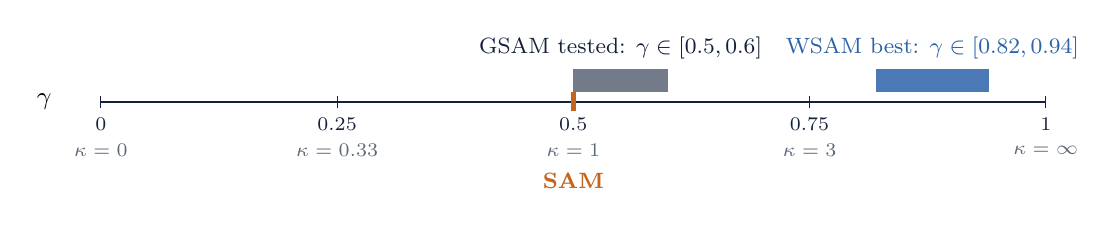
\begin{tikzpicture}[x=12cm]
  \draw[navy, thick] (0,0) -- (1,0);
  \foreach \g/\lab in {0/0, 0.25/0.25, 0.5/0.5, 0.75/0.75, 1/1} {
    \draw[navy] (\g,0.08) -- (\g,-0.08) node[below, font=\scriptsize] {\lab};
  }
  \foreach \g/\k in {0/0, 0.25/0.33, 0.5/1, 0.75/3, 1/\infty} {
    \node[font=\scriptsize, muted] at (\g,-0.62) {$\kappa=\k$};
  }
  \fill[navy!70, opacity=0.85] (0.5,0.12) rectangle (0.6,0.42);
  \node[font=\footnotesize, navy, above] at (0.55,0.42) {GSAM tested: $\gamma\in[0.5,0.6]$};
  \fill[flat, opacity=0.85] (0.82,0.12) rectangle (0.94,0.42);
  \node[font=\footnotesize, flat, above] at (0.88,0.42) {WSAM best: $\gamma\in[0.82,0.94]$};
  \draw[sharp, line width=1.6pt] (0.5,-0.12) -- (0.5,0.12);
  \node[font=\footnotesize\bfseries, sharp] at (0.5,-1.0) {SAM};
  \node[font=\small] at (-0.06,0) {$\gamma$};
\end{tikzpicture}\\[6pt]
\raggedright
GSAM's $\lambda\in[0,0.5]$ is $\kappa\in[1,1.5]$: \textbf{small} extra weights underperform projection.
WSAM's best $\kappa\approx4.6$--$16$: \textbf{large} weights, with decoupling, are competitive.
\source{Different settings (GSAM: ViT-B/32 on ImageNet; WSAM: CIFAR), so this is a reconciliation, not a head-to-head result.}
\end{frame}
\note{The most interesting point in this segment. Rewrite GSAM's rejected objective and it is exactly WSAM's with kappa = 1 + lambda. GSAM only searched lambda up to 0.5, i.e. gamma up to 0.6. WSAM's best gamma values are far outside that range. So the two papers do not really contradict each other.}

\begin{frame}{WSAM results}
\begin{columns}[T]
\begin{column}{0.55\textwidth}
\centering\small
\textbf{Top-1 error, \%} \mt{(Table 2, 5 seeds)}\\[3pt]
\begin{tabular}{@{}lcccc@{}}
\toprule
Model / data & SGDM & SAM & GSAM & WSAM\\
\midrule
ResNet-18 / C10 & 4.32 & 3.68 & 3.71 & \best{3.62}\\
ResNet-18 / C100 & 20.51 & 19.97 & 19.84 & \best{19.42}\\
WRN-28-10 / C10 & 3.73 & 2.94 & 2.91 & \best{2.74}\\
WRN-28-10 / C100 & 19.27 & 16.49 & 16.36 & \best{16.33}\\
\bottomrule
\end{tabular}\\[3pt]
{\scriptsize\mt{Several margins over GSAM are within one std (e.g.\ 16.33$\pm$0.26 vs 16.36$\pm$0.32).}}
\end{column}
\begin{column}{0.43\textwidth}
\centering\small
\textbf{Minima found} \mt{(ResNet-18, C10, Table 9)}\\[3pt]
\begin{tabular}{@{}lccc@{}}
\toprule
& Loss & Acc. & $\lambda_{\max}$\\
\midrule
SGDM & 0.0026 & 95.75 & 62.58\\
SAM & 0.0339 & 96.22 & \best{22.67}\\
WSAM & \best{0.0089} & \best{96.54} & 23.97\\
\bottomrule
\end{tabular}\\[4pt]
\raggedright\scriptsize
Nearly as flat as SAM, $\sim$4$\times$ lower training loss, better accuracy.
\end{column}
\end{columns}
\vspace{0.6em}
\begin{itemize}\small
  \item Setup: SGDM, 200 ep (vanilla 400), $\rho=0.2$; $\gamma\in\{0.82,0.88,0.94\}$; robust for $\gamma\in[0.8,0.95]$.
  \item Decoupling helps in 3 of 4 settings. \;ImageNet (3-ep DeiT-B fine-tune): \sh{no difference}, 18.01\% for SAM, GSAM, WSAM.
  \item Label noise: best at 20--60\%; at 80\% GSAM wins (79.09 vs 78.30).
\end{itemize}
\end{frame}
\note{Present the wins and the caveats together. Clearest win: WRN on CIFAR-10, 2.74 vs 2.91. Table 9 is a good discussion slide: WSAM puts MORE weight on sharpness yet ends up slightly sharper than SAM, with much lower loss and better accuracy. Ask: if flatness is about the same, why does WSAM generalize better? No settled answer; good lead-in to Eigen-SAM, which argues WHICH direction you flatten matters. Toy 2-D example (Sec. 4.2): sharp minimum loss 0.28 vs flat 0.36; SAM and gamma = 0.6 go to the sharp one, gamma = 0.95 finds the flat one. Adaptive and Fisher neighbourhoods did not help (2.90, 3.45). ESAM collapses at 80\% noise (32.29).}

% =====================================================================
\partsection{Part 4 $\cdot$ Eigen-SAM}{Luo, Truong, Pham, Harandi, Phung, Le $\cdot$ Monash \& VinAI $\cdot$ NeurIPS 2024}{Perturb where the sharpness actually is.}
% =====================================================================

\begin{frame}{SAM only sees curvature along the gradient}
Expand SAM's perturbed loss to second order, with $\hat\epsilon=\nabla L/\norm{\nabla L}$:
\[ L(w+\rho\hat\epsilon) \approx L(w) + \underbrace{\rho\norm{\nabla L}}_{\text{gradient-norm penalty}} + \underbrace{\tfrac{\rho^2}{2}\,\hat\epsilon^\top H\hat\epsilon}_{\text{curvature along }\hat\epsilon}
\qquad\text{and}\qquad
\hat\epsilon^\top H\hat\epsilon = \sum_i \lambda_i\cos^2\theta_i \]
\begin{columns}[T]
\begin{column}{0.48\textwidth}
\begin{exampleblock}{Aligned: $\hat\epsilon=\pm v_1$}
$\hat\epsilon^\top H\hat\epsilon=\lambda_1$: SAM directly penalizes the top eigenvalue.
\end{exampleblock}
\end{column}
\begin{column}{0.48\textwidth}
\begin{alertblock}{Misaligned: $\cos\theta_1\approx0$}
$\lambda_1$ barely appears: SAM flattens the \emph{wrong} directions.
\end{alertblock}
\end{column}
\end{columns}
\vspace{0.8em}
\centering
{\large Eigen-SAM's fix: \textbf{tilt the perturbation toward $v_1$}.}
\source{Simplified from the paper's third-order SDE analysis; the next slides give the formal version.}
\end{frame}
\note{Turning point of the talk: Parts 1 to 3 asked WHAT to minimize; Eigen-SAM asks WHICH DIRECTION to perturb. This slide is my simplified version of the paper's argument; it needs only a Taylor expansion. SAM implicitly minimizes three things: loss, a gradient-norm penalty, and curvature along the gradient direction. That curvature is a weighted sum of eigenvalues. It is lambda-1 only when the gradient is aligned with v1.}

\begin{frame}{Theory (1): $\lambda_1$ controls generalization}
\begin{block}{Theorem 3.1 (PAC-Bayes). With probability $\ge1-\delta$:}
\[ \begin{aligned}
f_{\mathcal D}(x) \le\; & f_S(x) + \sh{\frac{d\sigma^2}{2}\,\lambda_1\!\big(\nabla^2 f_S(x)\big)} + \frac{Cd^3\sigma^3}{6}\\
&+ \frac{L}{2\sqrt n}\sqrt{d\log\!\Big(1+\tfrac{\norm{x}^2}{d\sigma^2}\Big)+O(1)+2\log\tfrac1\delta+4\log(n+d)}
\end{aligned} \]
\end{block}
\begin{itemize}\setlength{\itemsep}{0.4em}
  \item Assumptions: loss bounded by $L$; third derivatives bounded by $C$; Gaussian weight noise does not lower test loss.
  \item Read it as: test loss $\le$ train loss $+$ \sh{(const)$\cdot\lambda_1$} $+$ higher order $+$ complexity.
  \item Unlike SAM's bound (``max loss in a ball''), $\lambda_1$ appears \textbf{explicitly}: a direct target.
\end{itemize}
\source{Proof: PAC-Bayes (Alquier et al., 2016) with Gaussian prior/posterior, union bound over priors, third-order Taylor expansion under Gaussian noise.}
\end{frame}
\note{d = number of parameters, n = number of samples, sigma = posterior noise scale. The key point for beginners: the eigenvalue term is explicit, so minimizing lambda-1 tightens the bound.}

\begin{frame}{Theory (2): what does SAM's drift minimize?}
Small learning rate $\eta$ $\Rightarrow$ training $\approx$ a noisy continuous path: \;$dX_t=\text{drift}\,dt+\text{noise}\,dW_t$.
\vspace{0.3em}
\begin{columns}[T]
\begin{column}{0.47\textwidth}
\begin{block}{2nd-order SDE (Compagnoni et al., 2023)}
\[ \text{drift} = -\nabla\big(f + \rho\,\mathbb E\norm{\nabla f_\gamma}\big) \]
SAM = a gradient-norm penalty. \mt{No eigenvalue term.}
\end{block}
\end{column}
\begin{column}{0.51\textwidth}
\begin{alertblock}{3rd-order SDE (Theorem 4.1)}
\[ \tilde f^{\mathrm{SAM}} = f + \rho\,\mathbb E\norm{\nabla f_\gamma} + \frac{\rho^2}{2}\,\mathbb E\!\left[\frac{\nabla f_\gamma^\top\nabla^2 f_\gamma\nabla f_\gamma}{\norm{\nabla f_\gamma}^2}\right] \]
Valid for $\rho=O(\eta^{1/3})$ (weak order-1, error $C\eta$).
\end{alertblock}
\end{column}
\end{columns}
\vspace{0.4em}
\begin{exampleblock}{Alignment and Corollary 4.1.1}
$\mathrm{Align}(\epsilon,v_1)\triangleq 1-\min_{s=\pm1}\norm{\epsilon/\norm{\epsilon}-s\,v_1}$.\quad
If $\mathrm{Align}\ge 1-O(\rho)$, the drift gains \;$\tfrac{\rho^2}{2}\nabla\,\mathbb E\,\lambda_1(\nabla^2 f_\gamma)$.\\
\textbf{SAM regularizes $\lambda_1$ only when it is well aligned.}
\end{exampleblock}
\end{frame}
\note{An SDE: drift is where SAM pushes on average; studying the drift tells you what SAM effectively minimizes. The older model only shows a gradient-norm penalty. The paper's model adds the rho-squared term, exactly the expansion from two slides ago in expectation over mini-batches (f\_gamma = mini-batch loss). Called third-order because differentiating that term needs third derivatives. Regime rho = O(eta\textasciicircum{}{1/3}) covers realistic rho values, unlike Wen et al. (2022), who need training time Theta(eta\textasciicircum{}-1 rho\textasciicircum{}-2) and rho exponentially smaller than eta. Assumptions: smoothness and growth conditions up to order 7, eigengap lambda1 > lambda2. With stronger alignment, 1 - O(rho\textasciicircum{}2), an extra rho E[s* lambda1 v1] term appears too.}

\begin{frame}{Evidence: alignment is poor in practice}
\begin{columns}[T]
\begin{column}{0.5\textwidth}
\begin{block}{Figure 1 (6-layer CNN, CIFAR-10)}
\begin{itemize}
  \item Alignment between SAM's perturbation and $v_1$ stays \textbf{low} throughout training.
  \item Consequently SAM does \textbf{not} efficiently drive $\lambda_1$ down.
\end{itemize}
\mt{\scriptsize Shown as curves only (95\% CI); no numbers in the text.}
\end{block}
\end{column}
\begin{column}{0.46\textwidth}
\centering\small
\textbf{Is SAM just a gradient-norm penalty?} \mt{(App.\ A, ResNet-18, CIFAR-10)}\\[4pt]
\begin{tabular}{@{}lc@{}}
\toprule
Method & Test acc.\\
\midrule
SAM & \best{95.5 $\pm$ 0.1}\\
Explicit grad.-norm reg.\ & 95.0 $\pm$ 0.2\\
Reverse-SAM ($-\epsilon$) & 94.4 $\pm$ 0.2\\
\bottomrule
\end{tabular}\\[6pt]
\raggedright\scriptsize
If SAM were only a gradient-norm penalty, the second row would match SAM. It does not.
\end{column}
\end{columns}
\end{frame}
\note{Point at the curves rather than quoting numbers. Teaching aside of mine: flipping epsilon to minus epsilon flips the sign of the rho*||grad|| term but leaves the rho-squared curvature term unchanged, so these baselines help separate the two effects.}

\begin{frame}{Eigen-SAM: estimate $v_1$, then tilt the perturbation}
\begin{columns}[T]
\begin{column}{0.5\textwidth}
\begin{algorithm}[H]
\caption{Power iteration (every $p$ steps)}
$\hat v \leftarrow$ random unit vector\;
\For{$q$ iterations}{
  $\hat v \leftarrow \nabla^2 f(x)\,\hat v$ \Comment*[r]{HVP}
  $\hat v \leftarrow \hat v/\norm{\hat v}$\;
}
\end{algorithm}
\vspace{-0.4em}
\begin{alertblock}{Perturbation (Eq.\ 8)}
\[ \epsilon = \frac{\nabla f_\gamma}{\norm{\nabla f_\gamma}} + \alpha\,\mathrm{sign}\big(\langle\nabla f_\gamma,\hat v\rangle\big)\,\hat v_\perp \]
\mt{\scriptsize $\hat v_\perp$: part of $\hat v$ orthogonal to the gradient. Then $\tilde x=x+\rho\epsilon$, $x\leftarrow x-\eta\nabla f_\gamma(\tilde x)$.}
\end{alertblock}
\end{column}
\begin{column}{0.48\textwidth}
\centering
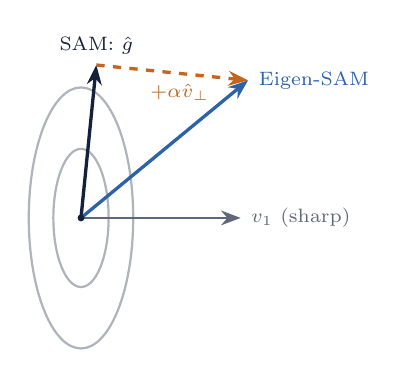
\begin{tikzpicture}[scale=0.78, >={Stealth[length=2.5mm]}]
  \foreach \k in {0.45,0.85} \draw[muted!50, thick] (0,0) ellipse ({\k} and {2.5*\k});
  \draw[->, muted, thick] (0,0) -- (2.6,0) node[right, font=\scriptsize] {$v_1$ (sharp)};
  \draw[->, navy, very thick] (0,0) -- (0.25,2.49) node[above, font=\scriptsize] {SAM: $\hat g$};
  \draw[->, sharp, very thick, dashed] (0.25,2.49) -- (2.72,2.24) node[pos=0.55, below, font=\scriptsize] {$+\alpha\hat v_\perp$};
  \draw[->, flat, very thick] (0,0) -- (2.72,2.24) node[right, font=\scriptsize] {Eigen-SAM};
  \fill[navy] (0,0) circle (1.6pt);
\end{tikzpicture}\\[2pt]
\begin{itemize}\small
  \item Defaults: $\alpha=0.2$, $p=100$, $q=5$
  \item Cost $\approx 2.05$--$2.10\times$ SGD; $<1\%$ extra at $p=1000$
  \item Prop.\ D.1: the tilt provably improves alignment
\end{itemize}
\end{column}
\end{columns}
\end{frame}
\note{Power iteration: repeatedly multiplying by H amplifies the top-eigenvalue component. Hessian-vector products via autodiff (Pearlmutter trick), about 1 to 2 gradients each; never build H (ResNet-18 has about 11M parameters, so H would have about 10\textasciicircum{}14 entries). Perturbation: start from SAM's direction and add only the orthogonal part of v-hat (the parallel part only changes length). The sign picks whichever of plus/minus v1 lies on the gradient's side, keeping it an ascent direction. Diagram: the gradient here is nearly orthogonal to v1; the tilt swings the perturbation toward v1 (drawn with alpha = 1 for visibility). Prop D.1 examples: omega = 0.8 allows alpha up to 3.43; omega = 0.9 up to 1.27. Convergence (Thm D.2): rate comparable to SAM, plus a non-vanishing beta\textasciicircum{}2(rho\textasciicircum{}2 + alpha\textasciicircum{}2) term, i.e. convergence to a neighbourhood of a stationary point.}

\begin{frame}{Running example: a badly aligned gradient}
$L=5w_1^2+0.5w_2^2$ at $w=(0.01,\,1)$: \;$g=(0.1,\,1)$, nearly orthogonal to $v_1$ \;($\cos\approx0.10$). \;True $\lambda_1=10$.\\[6pt]
\centering\small
\renewcommand{\arraystretch}{1.18}
\begin{tabular}{@{}lcccc@{}}
\toprule
& SGD & SAM ($\alpha=0$) & Eigen-SAM $\alpha=0.2$ & Eigen-SAM $\alpha=1$\\
\midrule
$|\cos(\epsilon, v_1)|$ & -- & 0.10 & 0.29 & 0.77\\
Curvature seen, $\hat\epsilon^\top H\hat\epsilon$ & -- & \sh{\textbf{1.09}} & 1.77 & \fl{\textbf{6.37}}\\
Update push on sharp coord.\ $w_1$ & 0.10 & 0.20 & 0.40 & 1.19\\
$\norm{\epsilon}$ & -- & 1.00 & 1.02 & 1.41\\
\bottomrule
\end{tabular}\\[8pt]
\raggedright
\takeaway{SAM ``sees'' a curvature of $\approx1.1$ where the truth is 10. The tilt makes the sharp direction visible.}
\mt{\small Question: $\norm{\epsilon}$ grows with $\alpha$. How would you show the gain comes from the direction, not the radius?}
\end{frame}
\note{My worked example: the model has nearly converged in the sharp direction but not in the flat one, so the gradient points mostly along the flat axis. At the paper's alpha = 0.2 the radius grows only about 2\%, so the effect is small in practice, but it is a good critical-thinking question.}

\begin{frame}{Eigen-SAM results}
\begin{columns}[T]
\begin{column}{0.6\textwidth}
\centering\small
\textbf{Test accuracy, \%} \mt{(Table 1, 95\% CI $\approx\pm0.1$--$0.2$)}\\[3pt]
\begin{tabular}{@{}llccc@{}}
\toprule
Model & Method & CIFAR-10 & CIFAR-100 & SVHN\\
\midrule
ResNet-18 & SGD & 94.8 & 74.6 & 96.1\\
 & SAM & 95.5 & 77.4 & 96.3\\
 & Eigen-SAM & \best{95.9} & \best{78.3} & \best{96.5}\\
\midrule
ResNet-50 & SAM & 95.6 & 79.0 & 96.4\\
 & Eigen-SAM & \best{96.2} & \best{79.7} & \best{96.6}\\
\midrule
WRN-28-10 & SAM & 96.5 & 82.0 & 96.4\\
 & Eigen-SAM & \best{96.8} & \best{82.8} & \best{96.7}\\
\bottomrule
\end{tabular}
\end{column}
\begin{column}{0.38\textwidth}
\small
\textbf{ViT-B/16 fine-tuning}\\[3pt]
\begin{tabular}{@{}lcc@{}}
\toprule
& C10 & C100\\
\midrule
SGD & 98.0 & 88.6\\
SAM & 98.4 & 89.5\\
Eigen-SAM & \best{98.5} & \best{89.8}\\
\bottomrule
\end{tabular}\\[8pt]
\begin{itemize}\setlength{\itemsep}{0.3em}
  \item $\alpha=0.2$ best: $+0.9$ over SAM (R18, C100)
  \item Smaller $\lambda_1$ \emph{and} trace (Fig.\ 3)
  \item \sh{Baselines: SGD and SAM only}
\end{itemize}
\end{column}
\end{columns}
\source{SGD momentum 0.9, batch 256, 200 ep, cosine LR, wd $5\!\times\!10^{-5}$; $\rho=0.05$ (C10, F-MNIST), $0.1$ (C100), $0.01$ (SVHN). Fashion-MNIST also reported.}
\end{frame}
\note{Eigen-SAM beats SAM in every cell. Largest gains on CIFAR-100 (about +0.7 to +0.9). Honest framing: gains are modest, often about the size of the confidence intervals. GSAM and WSAM are not baselines here; X-SAM's paper compares against all of them. SDE simulation (Sec 7.1): one-hidden-layer MLP on MNIST; the third-order SDE tracks discrete SAM more closely than the second-order one (plots only). Limitations to bridge: strong assumptions, v1 goes stale between refreshes, and the UPDATE is still the plain gradient at the perturbed point.}

% =====================================================================
\partsection{Part 5 $\cdot$ X-SAM}{Duan, Chen, Guan $\cdot$ Taiyuan University of Technology $\cdot$ arXiv preprint, 2026}{Look along the sharpest direction, but don't step along it.}
% =====================================================================

\begin{frame}{The update itself is often nearly orthogonal to $v_1$}
\begin{columns}[T]
\begin{column}{0.47\textwidth}
\begin{block}{Observation (Sec.\ 4.1)}
Angle between SAM's \textbf{update} gradient and $v_1$\\
\mt{\scriptsize (6-layer CNN, CIFAR-10, every 5 batches)}
\begin{itemize}
  \item $\approx$\textbf{45\%} of training: between $80^\circ$ and $100^\circ$
  \item $50^\circ$--$80^\circ$: updates drift toward \sh{sharper} regions
\end{itemize}
\end{block}
\mt{\small Eigen-SAM measured the angle of the \emph{perturbation}; X-SAM measures the angle of the \emph{update}.}
\end{column}
\begin{column}{0.5\textwidth}
Second-order effect of a step $\Delta w=-\eta g$:\\[4pt]
\textbf{Aligned} ($g=a v_1$):
\[ \Delta w^\top H\Delta w=(\eta a)^2\lambda_1 \]
\textbf{General}, component along $v_1$:
\[ (\Delta w^\top H\Delta w)_{v_1} = \lambda_1\eta^2\langle g,v_1\rangle^2 \]
\mt{\small Why not optimize the angle directly? Costly, and it conflicts with the loss gradient $\Rightarrow$ decompose instead.}
\end{column}
\end{columns}
\end{frame}
\note{X-SAM builds directly on Eigen-SAM: same power iteration, same training recipe, even the same variable names. Present it as Eigen-SAM's sequel, and as a preprint (no venue listed). Bridge: Eigen-SAM fixed where SAM looks; X-SAM asks what if the step we actually take walks toward sharp regions. Angles computed from per-layer flattened, normalized gradients and eigenvectors, concatenated. Objectives like max theta(w) or min f - lambda cos theta (Eq. 7) are dismissed, echoing GSAM's rejection of f\_p + lambda h. Generalization link: cites Eigen-SAM's PAC-Bayes corollary rather than deriving its own.}

\begin{frame}{X-SAM: shrink the update's component along $v_1$}
\begin{columns}[T]
\begin{column}{0.52\textwidth}
\begin{algorithm}[H]
\caption{X-SAM}
\For{$t=1,\dots,T$}{
  \lIf{$t \bmod p = 1$}{$\hat v\leftarrow$ PowerIteration$(q)$}
  $w^{\mathrm{adv}} \leftarrow w_t + \rho\,\nabla f(w_t)/\norm{\nabla f(w_t)}$\;
  $\hat g \leftarrow \nabla f(w^{\mathrm{adv}})/\norm{\nabla f(w^{\mathrm{adv}})}$\;
  $g_X \leftarrow (I-\alpha\hat v\hat v^\top)\,\hat g = \hat g - \alpha\langle\hat g,\hat v\rangle\hat v$\;
  $w_{t+1}\leftarrow w_t-\eta\,g_X$\;
}
\end{algorithm}
\mt{\small $\alpha=0.2$; stable for $\alpha\in[0.1,0.4]$; $p,q$ not given in the main text.}
\end{column}
\begin{column}{0.46\textwidth}
\centering
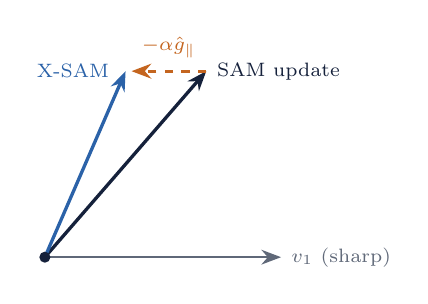
\begin{tikzpicture}[scale=1.25, >={Stealth[length=2.5mm]}]
  \draw[->, muted, thick] (0,0) -- (2.4,0) node[right, font=\scriptsize] {$v_1$ (sharp)};
  \draw[->, navy, very thick] (0,0) -- (1.64,1.89) node[right, font=\scriptsize] {SAM update};
  \draw[->, sharp, very thick, dashed] (1.64,1.89) -- (0.88,1.89) node[midway, above=1pt, font=\scriptsize] {$-\alpha\hat g_\parallel$};
  \draw[->, flat, very thick] (0,0) -- (0.82,1.89) node[left=2pt, font=\scriptsize] {X-SAM};
  \fill[navy] (0,0) circle (1.6pt);
\end{tikzpicture}\\[6pt]
\small
\renewcommand{\arraystretch}{1.15}
\begin{tabular}{@{}lll@{}}
\toprule
Method & Decomposes & Used in\\
\midrule
GSAM & $\nabla f$ vs $\nabla\fp$ & update\\
Eigen-SAM & $v_1$ vs $\nabla f$ & perturbation\\
X-SAM & $\nabla\fp$ vs $v_1$ & update\\
\bottomrule
\end{tabular}
\end{column}
\end{columns}
\vspace{0.3em}
\centering
{\large Eigen-SAM: \textbf{look} along $v_1$. \quad X-SAM: don't \textbf{step} along $v_1$.}
\end{frame}
\note{I present the projector form P = I - alpha v v\textasciicircum{}T from the convergence theorem: it shrinks the update's component along v1 by a factor (1 - alpha). The paper's Eq. 11 has an extra sign factor that, combined with g\_parallel, makes the update depend on whether power iteration returned +v1 or -v1 (see critical-reading slide). The table shows the same decomposition trick used three ways. The two eigenvector methods are complementary and could in principle be combined: good closing question.}

\begin{frame}{Running example and theory intuition}
\begin{columns}[T]
\begin{column}{0.47\textwidth}
\textbf{Toy} \mt{\small($w=(0.05,1)$, $\rho=0.1$; $g$ at $63^\circ$ to $v_1$)}\\[4pt]
\footnotesize
\renewcommand{\arraystretch}{1.15}
\begin{tabular}{@{}lccc@{}}
\toprule
& SAM & $\alpha=0.2$ & $\alpha=0.5$\\
\midrule
angle to $v_1$ & $49^\circ$ & $55^\circ$ & $66.5^\circ$\\
curvature along step & \sh{4.88} & 3.93 & \fl{2.43}\\
\bottomrule
\end{tabular}\\[6pt]
\mt{\scriptsize In a quadratic $H$ is constant, so this shows the \emph{direction} effect only.}
\end{column}
\begin{column}{0.51\textwidth}
\textbf{Why it limits $\lambda_1$} (eigenvalue perturbation):
\[ \Delta\lambda_1 \approx v_1^\top\Delta H\,v_1 \approx \langle\nabla\lambda_1,\Delta w\rangle \]
\begin{block}{Theorem 5.3 (informal)}
If the step has no $v_1$ component ($v_1^\top g=0$) and $\nabla\lambda_1$ lies mostly along $v_1$:
\[ |\Delta\lambda_1|\le\eta\varepsilon\norm{g}+O(\eta^2\norm{g}^2)+O\!\big(\tfrac{\eta^2\norm{g}^2}{\gamma}\big) \]
\end{block}
\mt{\small Shows $\lambda_1$ is kept from \emph{growing}; no separate generalization bound.}
\end{column}
\end{columns}
\vspace{0.2em}
\footnotesize\textbf{Convergence (Thm 5.1):} \;$\tfrac1T\sum_t\mathbb E\norm{\nabla f}^2\le c_1\big(\tfrac{\beta\Delta}{T}+\sqrt{\tfrac{\beta\Delta\sigma^2}{T}}\big)+c_2(1+2\alpha^2)$ \;\mt{(last term does not vanish)}
\end{frame}
\note{Toy (mine): X-SAM steers the step away from the sharp axis, so less of the move happens in the lambda = 10 direction. Real lambda1 changes need third derivatives, which the theorems handle. Theorem 5.2 (eigenvalue perturbation bound) assumes eigengap gamma = lambda1 - lambda2 > 0, ||Delta H|| = s < gamma: lambda1(H + Delta H) <= lambda1(H) + v1\textasciicircum{}T Delta H v1 + 4(||H|| + s)s/(gamma - s). Theorem 5.3 assumes f in C\textasciicircum{}4 with bounded 3rd and 4th derivatives and a simple top eigenvalue. Convergence assumptions: beta-smooth, alpha in [0,2], unbiased gradients with variance sigma\textasciicircum{}2. Like Eigen-SAM, convergence is to a neighbourhood. Section 5.2 is titled "Eigenvalue Decrease Enhances Generalization" but contains no bound of its own.}

\begin{frame}{X-SAM results (top-1 accuracy, \%)}
\centering\footnotesize
\setlength{\tabcolsep}{4.5pt}
\renewcommand{\arraystretch}{1.1}
\begin{tabular}{@{}lccccc@{\hspace{1.2em}}ccccc@{}}
\toprule
& \multicolumn{5}{c}{CIFAR-10} & \multicolumn{5}{c}{CIFAR-100}\\
\cmidrule(lr){2-6}\cmidrule(lr){7-11}
Method & R18 & R50 & WRN & AlexNet & Avg & R18 & R50 & WRN & AlexNet & Avg\\
\midrule
SAM & 93.64 & 92.33 & 95.01 & 88.66 & 92.41 & 74.00 & 72.01 & 77.96 & 60.26 & 71.06\\
WSAM & 93.01 & 91.68 & 94.23 & 90.08 & 92.25 & 73.65 & 71.04 & 77.19 & 65.90 & 71.95\\
GSAM & 93.80 & 92.16 & 94.67 & 88.59 & 92.31 & 73.55 & 71.61 & 78.15 & 60.14 & 70.86\\
Eigen-SAM & 93.82 & 92.57 & 95.11 & 88.79 & 92.57 & 73.74 & 71.90 & 78.20 & 60.49 & 71.08\\
\textbf{X-SAM} & \best{94.71} & \best{93.76} & \best{95.53} & \best{90.73} & \best{93.68} & \best{74.10} & \best{74.08} & \best{78.23} & \best{68.82} & \best{73.81}\\
\bottomrule
\end{tabular}\\[6pt]
\raggedright
\begin{itemize}\small\setlength{\itemsep}{0.2em}
  \item X-SAM wins every column on CIFAR-10 and CIFAR-100. \;Fashion-MNIST gains are small ($\approx$0.2--0.3).
  \item \sh{AlexNet} (no batch norm, no residuals) drives the averages: CIFAR-100 $60.3\to68.8$.
  \item Excluding AlexNet, CIFAR-100 gains over SAM: $+0.1$, $+2.1$, $+0.3$, several within one std.
  \item Reported: faster, less oscillating $\lambda_1$ decrease; smaller $\lambda_1$ and trace than SAM.
\end{itemize}
\source{Same recipe as Eigen-SAM (SGD, LR 0.1 cosine, batch 256, 200 ep); 3 runs; single RTX 4090. No SGD baseline.}
\end{frame}
\note{Training dynamics (Fig. 2): training loss falls quickly early; lambda1 drops faster with fewer oscillations and stays low, even while training loss rises slightly, the GSAM theme of accepting slightly higher loss for flatness. alpha sensitivity: best 0.2, +1.07 over SAM. No ablation of p and q, no runtime numbers; the conclusion admits eigenvector estimation cost is non-negligible. Future work: reduce overhead, scale to large models.}

\begin{frame}{Reading a preprint critically}
\begin{columns}[T]
\begin{column}{0.49\textwidth}
\begin{alertblock}{Method}
\begin{itemize}\small
  \item \textbf{Eq.\ 11 sign issue}: the extra sign factor makes the update depend on whether power iteration returned $+v_1$ or $-v_1$. The projector form has no such problem.
  \item \textbf{Normalized step}: $\hat g=g/\norm g$ fixes step length to $\eta$. Not ablated; part of the gain may come from this.
\end{itemize}
\end{alertblock}
\begin{alertblock}{Reporting}
\begin{itemize}\small
  \item Averages inconsistent in places; gain figures differ between intro and Sec.\ 6.2.
  \item 3 seeds; $p,q$ missing; no runtime.
\end{itemize}
\end{alertblock}
\end{column}
\begin{column}{0.49\textwidth}
\begin{alertblock}{Baselines}
\begin{itemize}\small
  \item Same recipe as Eigen-SAM, yet R18/C10:\\
  SAM \textbf{93.64} here vs \textbf{95.5} in Eigen-SAM's paper.
  \item Even X-SAM's 94.71 is below SAM's number there.
  \item WSAM run with $\rho=2$--$4$, vs 0.2 in its own paper.
\end{itemize}
\end{alertblock}
\vspace{0.4em}
\begin{exampleblock}{Verdict}
\centering Elegant, well-motivated idea.\\ Preliminary evidence.
\end{exampleblock}
\end{column}
\end{columns}
\end{frame}
\note{Frame this as a two-minute how-to-read-a-preprint exercise, not an attack. Numerical check of Eq. 11 on the toy example: v = +v1 and v = -v1 give different updates, (0.52, 0.75) vs (0.79, 0.75). The text also says the update follows "Eq. (5)", which is a curvature expression, not an update rule. Also: the abstract's "<= 90 degrees" claim is not cleanly derived; the body uses ranges. WSAM fails to converge on Fashion-MNIST/AlexNet, probably due to the large rho. Some bolded "best" entries are not best (GSAM beats X-SAM on F-MNIST WRN). Ask the class: what ablation would separate the normalization effect from the eigenvector correction?}

% =====================================================================
\partsection{Wrap-up}{Five methods, one recipe}{What changed, and what is still open?}
% =====================================================================

\begin{frame}{Five methods side by side}
\centering\small
\renewcommand{\arraystretch}{1.3}
\begin{tabular}{@{}>{\bfseries}l>{\raggedright}p{2.0cm}>{\raggedright}p{2.1cm}>{\raggedright}p{2.0cm}>{\raggedright}p{2.1cm}>{\raggedright\arraybackslash}p{2.1cm}@{}}
\toprule
& SAM & GSAM & WSAM & Eigen-SAM & X-SAM\\
\midrule
Venue & ICLR 2021 & ICLR 2022 & KDD 2023 & NeurIPS 2024 & arXiv 2026\\
Changes & defines the objective & \textbf{update}: ascent on $\nabla f_\perp$ & \textbf{objective}: weight $\gamma$ & \textbf{perturbation}: tilt to $v_1$ & \textbf{update}: shrink $v_1$ part\\
Sharpness & worst loss in $\rho$-ball & $h\approx\tfrac12\rho^2\lambda_1$ & weighted $\tilde L$ & $\lambda_1$ via alignment & $\lambda_1$ via update angle\\
Extra knobs & $\rho$ & $\alpha$, $\rho_t$ & $\gamma$ & $\alpha,p,q$ & $\alpha,p,q$\\
Cost vs SGD & $2\times$ & $\approx2\times$ & $\approx2\times$ & $2.05$--$2.1\times$ & $>2\times$\\
Evidence & very broad & ImageNet ViT/Mixer & CIFAR & CIFAR, ViT FT & CIFAR (prelim.)\\
\bottomrule
\end{tabular}
\end{frame}
\note{One table summarizing everything. Read it row by row: what each changes, what notion of sharpness it uses, what it costs, how strong the evidence is.}

\begin{frame}{The storyline in three sentences}
\begin{enumerate}\setlength{\itemsep}{1.4em}
  \item[\textbf{1.}] \textbf{SAM.} Flat minima generalize, so minimize the \emph{worst-case} loss in a neighbourhood.
  \item[\textbf{2.}] \textbf{GSAM \& WSAM.} The worst-case loss mixes depth with flatness, so separate the sharpness term and control it: by \emph{projection} (GSAM) or by \emph{weighting} (WSAM).
  \item[\textbf{3.}] \textbf{Eigen-SAM \& X-SAM.} Sharpness really means $\lambda_1$, which lives along one direction $v_1$: \emph{look} along $v_1$ (Eigen-SAM) and don't \emph{step} along it (X-SAM).
\end{enumerate}
\end{frame}
\note{If students remember one slide, it should be this one.}

{
\metroset{background=dark}
\begin{frame}[standout]
Every method here assumes flatness,\\ specifically $\lambda_1$, is the right target.\\[1em]
\alert{Is it?}\\[1.2em]
{\normalsize\normalfont
Kaur, Cohen \& Lipton: \emph{On the Maximum Hessian Eigenvalue and Generalization}\\
Dinh et al.\ (2017): \emph{Sharp Minima Can Generalize for Deep Nets}}
\end{frame}
}
\note{Closing question. Dinh et al. show sharpness measures can be changed by reparameterizing a network without changing what it computes. Kaur et al. (on the reading list) examine whether lambda-max reliably tracks generalization. Also on the reading list: Bahri et al. show SAM helps language models; Chaudhari et al.'s Entropy-SGD is an earlier flatness-seeking method that GSAM benchmarks against.}

\begin{frame}[allowframebreaks]{References}
\footnotesize
\begin{itemize}\setlength{\itemsep}{0.35em}
  \item P.~Foret, A.~Kleiner, H.~Mobahi, B.~Neyshabur. Sharpness-Aware Minimization for Efficiently Improving Generalization. \emph{ICLR}, 2021. arXiv:2010.01412.
  \item J.~Zhuang, B.~Gong, L.~Yuan, Y.~Cui, H.~Adam, N.~Dvornek, S.~Tatikonda, J.~Duncan, T.~Liu. Surrogate Gap Minimization Improves Sharpness-Aware Training. \emph{ICLR}, 2022. arXiv:2203.08065.
  \item Y.~Yue, J.~Jiang, Z.~Ye, N.~Gao, Y.~Liu, K.~Zhang. Sharpness-Aware Minimization Revisited: Weighted Sharpness as a Regularization Term. \emph{KDD}, 2023. arXiv:2305.15817.
  \item H.~Luo, T.~Truong, T.~Pham, M.~Harandi, D.~Phung, T.~Le. Explicit Eigenvalue Regularization Improves Sharpness-Aware Minimization. \emph{NeurIPS}, 2024. arXiv:2501.12666.
  \item H.~Duan, Y.~Chen, L.~Guan. X-SAM: Boosting Sharpness-Aware Minimization with Dominant-Eigenvector Gradient Correction. arXiv:2601.10251, 2026.
  \item S.~Kaur, J.~Cohen, Z.~C.~Lipton. On the Maximum Hessian Eigenvalue and Generalization. \emph{ICBINB Workshop, PMLR}, 2023.
  \item D.~Bahri, H.~Mobahi, Y.~Tay. Sharpness-Aware Minimization Improves Language Model Generalization. \emph{ACL}, 2022.
  \item P.~Chaudhari et al. Entropy-SGD: Biasing Gradient Descent into Wide Valleys. \emph{ICLR}, 2017.
  \item L.~Dinh, R.~Pascanu, S.~Bengio, Y.~Bengio. Sharp Minima Can Generalize for Deep Nets. \emph{ICML}, 2017.
  \item N.~S.~Keskar et al. On Large-Batch Training for Deep Learning: Generalization Gap and Sharp Minima. \emph{ICLR}, 2017.
  \item J.~Kwon, J.~Kim, H.~Park, I.~K.~Choi. ASAM: Adaptive Sharpness-Aware Minimization. \emph{ICML}, 2021.
  \item E.~M.~Compagnoni et al. An SDE for Modeling SAM: Theory and Insights. \emph{ICML}, 2023.
  \item K.~Wen, T.~Ma, Z.~Li. How Does Sharpness-Aware Minimization Minimize Sharpness? \emph{ICLR}, 2023.
\end{itemize}
\end{frame}

{
\metroset{background=dark}
\begin{frame}[standout]
Thank you\\[0.6em]
{\normalsize Questions?}
\end{frame}
}

% =====================================================================
\appendix
\partsection{Backup}{Full statements and hyperparameters}{}
% =====================================================================

\begin{frame}{Backup: SAM Theorem 2 (full statement, App.\ A.1)}
For any $\rho>0$ and any distribution $\mathcal D$, with probability $1-\delta$ over $S\sim\mathcal D$:
\[
L_{\mathcal D}(w) \le \max_{\norm{\epsilon}_2\le\rho} L_S(w+\epsilon)
+ \sqrt{\frac{k\log\!\Big(1+\frac{\norm{w}_2^2}{\rho^2}\big(1+\sqrt{\tfrac{\log n}{k}}\big)^2\Big) + 4\log\frac n\delta + \tilde O(1)}{n-1}}
\]
\begin{itemize}
  \item $n=|S|$, $k$ = number of parameters.
  \item Assumes $L_{\mathcal D}(w)\le\mathbb E_{\epsilon_i\sim\mathcal N(0,\rho)}[L_{\mathcal D}(w+\epsilon)]$: Gaussian perturbation does not decrease test error. Expected at a final solution, not for arbitrary $w$.
  \item Proof: PAC-Bayes (McAllester 1999), Gaussian prior and posterior, predefined grid of prior variances with a union bound (Langford \& Caruana), chi-square concentration (Laurent \& Massart).
\end{itemize}
\end{frame}

\begin{frame}{Backup: hyperparameters at a glance}
\centering\small
\renewcommand{\arraystretch}{1.3}
\begin{tabular}{@{}l>{\raggedright}p{8.4cm}>{\raggedright\arraybackslash}p{3.4cm}@{}}
\toprule
Method & Recommended / reported values & Source\\
\midrule
SAM & $\rho=0.05$ default; grid $\{0.01,\dots,0.5\}$; $p=2$ & Foret et al., App.\ C.3, C.5\\
GSAM & $\rho$: 0.04$\to$0.02 (ResNet), up to 0.7 (ViT/Mixer); $\alpha$: 0.005--0.01 (ResNet), 0.01--1.0 (ViT/Mixer) & Zhuang et al., Table 4\\
WSAM & $\rho=0.2$ (CIFAR); $\gamma\in[0.8,0.95]$, start at 0.9 & Yue et al., Table 3, Fig.\ 3\\
Eigen-SAM & $\alpha=0.2$, $p=100$, $q=5$ & Luo et al., Sec.\ 5--7\\
X-SAM & $\alpha=0.2$ (stable 0.1--0.4); $\rho$ as SAM; $p,q$ in appendix & Duan et al., Sec.\ 6\\
\bottomrule
\end{tabular}
\end{frame}

\end{document}